\documentclass[12pt,a4paper]{article}
\usepackage[polish]{babel}
\usepackage[T1]{fontenc}
\usepackage[utf8x]{inputenc}
\usepackage{hyperref}
\usepackage{url}
\usepackage[]{algorithm2e}
\SetKw{KwBy}{by}
\SetKwProg{try}{try}{:}{}
\SetKwProg{catch}{catch}{:}{end}

\usepackage{graphicx}
\usepackage{color}
\usepackage{listings}
\usepackage{mathtools}

\usepackage{pgfplots}
\pgfplotsset{width=13cm,compat=1.9}
\usepgfplotslibrary{external}

\lstloadlanguages{% Check Dokumentation for further languages ...
	C,
	C++,
	csh,
	Java
}

\definecolor{red}{rgb}{0.6,0,0} % for strings
\definecolor{blue}{rgb}{0,0,0.6}
\definecolor{green}{rgb}{0,0.8,0}
\definecolor{cyan}{rgb}{0.0,0.6,0.6}

\lstset{
	language=csh,
	basicstyle=\footnotesize\ttfamily,
	numbers=left,
	numberstyle=\tiny,
	numbersep=5pt,
	tabsize=2,
	extendedchars=true,
	breaklines=true,
	frame=b,
	stringstyle=\color{blue}\ttfamily,
	showspaces=false,
	showtabs=false,
	xleftmargin=17pt,
	framexleftmargin=17pt,
	framexrightmargin=5pt,
	framexbottommargin=4pt,
	commentstyle=\color{green},
	morecomment=[l]{//}, %use comment-line-style!
	morecomment=[s]{/*}{*/}, %for multiline comments
	showstringspaces=false,
	morekeywords={ abstract, event, new, struct,
		as, explicit, null, switch,
		base, extern, object, this,
		bool, false, operator, throw,
		break, finally, out, true,
		byte, fixed, override, try,
		case, float, params, typeof,
		catch, for, private, uint,
		char, foreach, protected, ulong,
		checked, goto, public, unchecked,
		class, if, readonly, unsafe,
		const, implicit, ref, ushort,
		continue, in, return, using,
		decimal, int, sbyte, virtual,
		default, interface, sealed, volatile,
		delegate, internal, short, void,
		do, is, sizeof, while,
		double, lock, stackalloc,
		else, long, static,
		enum, namespace, string},
	keywordstyle=\color{cyan},
	identifierstyle=\color{red},
}
\usepackage{caption}
\DeclareCaptionFont{white}{\color{white}}
\DeclareCaptionFormat{listing}{\colorbox{blue}{\parbox{\textwidth}{\hspace{15pt}#1#2#3}}}
\captionsetup[lstlisting]{format=listing,labelfont=white,textfont=white, singlelinecheck=false, margin=0pt, font={bf,footnotesize}}


\addtolength{\hoffset}{-1.5cm}
\addtolength{\marginparwidth}{-1.5cm}
\addtolength{\textwidth}{3cm}
\addtolength{\voffset}{-1cm}
\addtolength{\textheight}{2.5cm}
\setlength{\topmargin}{0cm}
\setlength{\headheight}{0cm}

\begin{document}
	
	\title{Systemy sztucznej inteligencji\\\small{dokumentacja projektu Digit Recognizer}}
	\author{
	Jambor Daniel\\
	Grupa 2D
	\and
	Kozieł Wojtek\\
	Grupa 2D
	\and
	Matula Kamil\\
	Grupa 2D}

	\date{\today}

	\maketitle
	\newpage
	
\section*{Część I}
\subsection*{Opis programu}
\hspace{20pt}Program \textit{\textbf{Digit Recognizer}} służy do rozpoznawania ręcznie napisanych działań i wyświetlania ich wyniku. Użytkownik pisze na specjalnym polu liczby naturalne oraz dowolne z czterech zaimplementowanych znaków arytmetycznych (odpowiadających działaniom dodawania, odejmowania, dzielenia i mnożenia), a program wyświetla końcowy wynik podanego wyrażenia. Program korzysta z bazy danych ,,MNIST'', składającej się łącznie z 70 000 ręcznie napisanych cyfr, oraz z autorskiej bazy cyfr i oznaczeń matematycznych.	
\vspace{10pt}	
\subsection*{Instrukcja obsługi}
\hspace{20pt}Po uruchomieniu pliku wykonawczego \textit{DigitRecognizer.exe}, użytkownik powinien zobaczyć poniższy interfejs graficzny:

	\begin{figure}[h!]
	\centering
	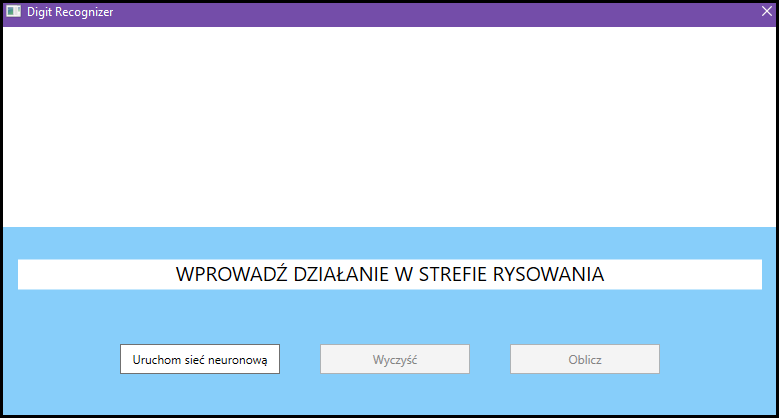
\includegraphics[height=8.5cm]{graphics/app.png}
	\end{figure}

\noindent Jak widać na zamieszczonym wyżej zrzucie ekranu aplikacja składa się z:
	\begin{itemize}
	\item białego pola (tzw. ,,strefy rysowania''), na którym użytkownik może zapisywać działania,
	\item szerokiego pola tekstowego, gdzie wyświetlane są wszystkie komunikaty związane z działaniem programu włącznie z wynikiem zapisanego wyrażenia,
	\item przycisku ,,Uruchom sieć neuronową'', który jako jedyny jest dostępny po uruchomieniu programu - pozwala on zbudować sieć neuronową i wczytać wcześniej wyuczone wagi,
	\item przycisku ,,Wyczyść'', który czyści zawartość strefy rysowania,
	\item przycisku ,,Oblicz'', który zleca sieci neuronowej pobranie narysowanych przez użytkownika cyfr i znaków, a także zwraca obliczony wynik.
	\end{itemize}
	

Po wciśnięciu przycisku ,,Uruchom sieć neuronową'' w polu tekstowym pojawi się informacja o tym, że sieć jest już gotowa. Ponadto przycisk ten stanie się nieaktywnym, a pozostałe dwa uaktywnią się, co widać na poniższym obrazku:

	\begin{figure}[h!]
	\centering
	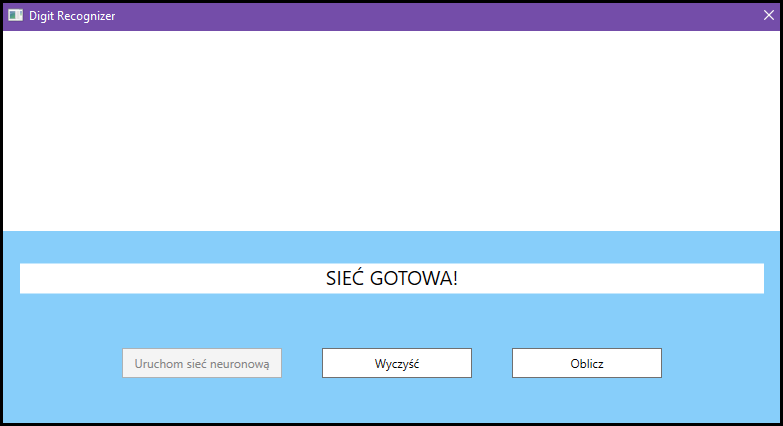
\includegraphics[height=8.5cm]{graphics/app2.png}
	\end{figure}
	
	\vspace{40pt}
W celu obliczenia wartości pewnego wyrażenia wystarczy napisać je w strefie rysowania, a następnie wcisnąć przycisk ,,Oblicz'' np.:

	\begin{figure}[h!]
	\centering
	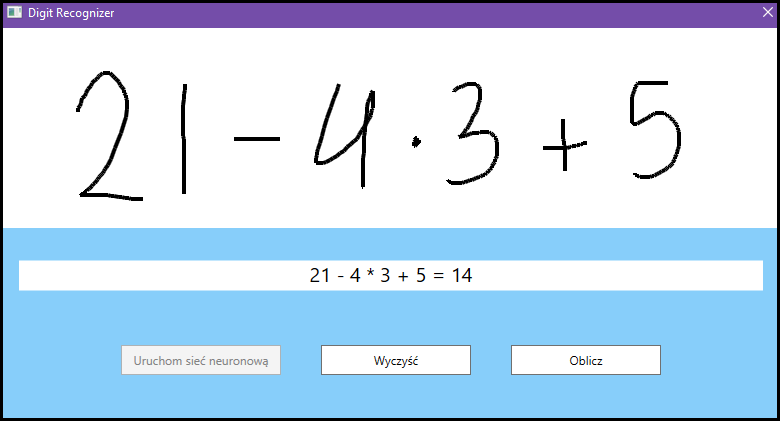
\includegraphics[height=8.5cm]{graphics/app3.png}
	\end{figure}
\subsection*{Dodatkowe informacje}
\subsubsection*{Wymagania i zabezpieczenia}
    \hspace{20pt}Do prawidłowego działania aplikacji wymagany jest plik \textit{weights.txt}, który powinien znajdować się w tym samym folderze, co plik \textit{DigitRecognizer.exe}. Zawiera on konfigurację sieci (współczynnik $\alpha$ funkcji aktywacji oraz ilość neuronów na poszczególnych warstwach), a także wagi synaps wejściowych każdej warstwy. W przypadku nieodnalezienia pliku z wagami lub niepoprawnej zawartości tego pliku pojawi się komunikat \textit{,,NIE ZNALEZIONO PRAWIDŁOWEGO PLIKU Z WAGAMI!''}. Program został także zabezpieczony przed możliwością dzielenia liczby przez zero co widać poniżej: 
    \begin{figure}[h!]
	\centering
	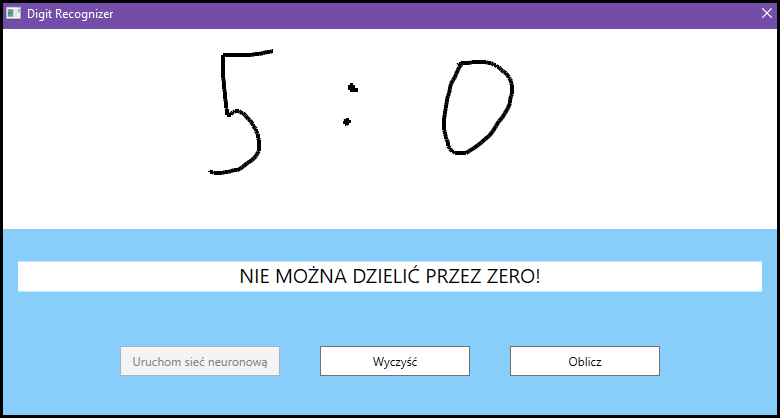
\includegraphics[height=7.5cm]{graphics/app4.png}
	\end{figure}
    
    \noindent oraz przed niepoprawnym zapisem (tj. obecnością znaku arytmetycznego na początku wyrażenia, jego końcu lub obok innego znaku):
    
    \begin{figure}[h!]
	\centering
	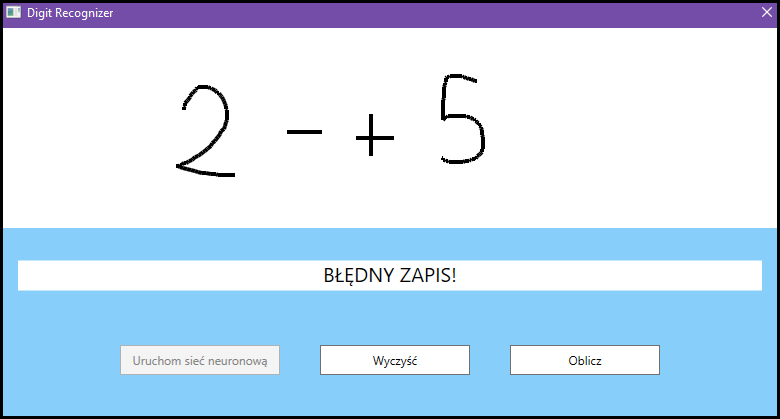
\includegraphics[height=7.5cm]{graphics/app5.png}
	\end{figure}
\subsubsection*{Przygotowanie sieci neuronowej}
    \hspace{20pt}Sama aplikacja nie wymaga niczego oprócz dwóch wspomnianych plików, jednakże sieć neuronowa musiała wcześniej zostać nauczona rozpoznawania cyfr, zanim mogła zostać użyta w programie. W oddzielnym folderze projektu o podtytule \textit{Learning Place} znajduje się zestaw plików źródłowych napisanych w języku C\#, a także folder \textit{Datasets} zawierający bazę MNIST oraz bazę autorską. Aby lepiej nauczyć sieć należy zmodyfikować ustawienia zapisane w metodzie \textit{Main} w pliku \textit{Program.cs}. Możliwe jest też douczenie sieci wstępnie nauczonej, dzięki zaimplementowanej funkcji wczytywania wag. Po nauczaniu plik z wagami powinien zostać skopiowany z folderu bieżącego do folderu, w którym znajduje się plik wykonawczy \textit{DigitRecognizer.exe}.
\subsubsection*{Dodatkowe technologie i ich niedokładności}
	\hspace{20pt}Do stworzenia pola zwanego ,,strefą rysowania'' wykorzystano klasę \textit{Canvas}, czyli obszar, na którym można pozycjonować elementy podrzędne, oraz klasę \textit{Line} z przestrzeni nazw \textit{Shapes}, z której pomocą zaimplementowano możliwość rysowania linii z użyciem myszy. \\W połączeniu z algorytmem wycinającym każdy znak lub cyfra rozpoznawane są osobno.
	
	\vspace{5pt} Niestety połączenie Canvas oraz zaimplementowanych przez nas algorytmów do przetwarzania otrzymanego obrazu niesie za sobą pewne ryzyko wykrycia przez algorytm pojedynczych pikseli odłączonych od znaku, powstałych w skutek poszarpania linii rysowania. Piksele te znajdują się nad lub pod znakiem i mają niewielki wpływ na dokładność odczytywania znaku.
	
    \vspace{5pt} Algorytm przetwarzający obraz wykorzystuje klasę \textit{Graphics} z przestrzeni nazw \\ \textit{System.Drawing}, której właściwości pozwoliły na wycięcie oraz przeskalowanie obrazów bez ich zniekształcenia. Dzięki strukturze \textit{Rectangle} z tej przestrzeni możliwe było wycięcie figur z użyciem tylko punktów początkowych i końcowych cięcia. 
	
    \newpage
\section*{Część II}
\subsection*{Opis działania sieci neuronowej} 
	\hspace{20pt} Jak zostało wcześniej wspomniane program opiera się na sztucznej sieci neuronowej (SSN), czyli matematycznym modelu sieci nerwowej działającej w mózgu. Podobnie jak ludzka sieć neuronowa, SSN zbudowana jest z neuronów ułożonych w warstwy. Każda komórka nerwowa danej warstwy połączona jest ze wszystkimi komórkami warstwy poprzedniej i warstwy następnej za pomocą synaps posiadających pewne losowo zainicjowane wagi w postaci liczb. Są one modyfikowane w procesie uczenia sieci neuronowej.
	
	\vspace{5pt}
	Pierwszą warstwę sieci, odpowiedzialną za przyjmowanie danych wejściowych, nazywamy warstwą wejściową. Analogicznie ostatnia warstwa sieci to warstwa wyjściowa, odpowiadająca za zwracanie wyniku. Pomiędzy nimi mogą (lecz nie muszą) znajdować się tzw. warstwy ukryte. Zadaniem projektanta sieci neuronowej jest znalezienie optymalnej ilości i wielkości tych warstw, dzięki czemu nauczanie będzie przebiegało efektywnie. Z kolei ilość neuronów na warstwach skrajnych zależy od tego, ile cech posiada obiekt wejściowy oraz do ilu klas można go zaklasyfikować na wyjściu - w przypadku tego projektu jest to 784 neuronów wejściowych (z każdego piksela pobieramy osobną wartość) oraz 14 neuronów wyjściowych (tyle różnych znaków można uzyskać dzięki rozpoznawaniu).
	
	\vspace{5pt}
	Każdy z neuronów przyjmuje pewną wartość na wejściu, a następnie przetwarza ją dzięki funkcji aktywacji. Sygnał wejściowy i-tego neuronu k-tej warstwy można opisać równaniem:
	
	\begin{equation*}
	    s^k_i = \sum_{j=1}^{n}w^k_{ij} y^{k-1}_{j} + b,
	\end{equation*}
	
	\noindent gdzie $w^k_{ij}$ - waga synapsy pomiędzy i-tym neuronem k-tej warstwy a j-tym neuronem warstwy poprzedniej, $y^{k-1}_{j}$ - wartość sygnału wyjściowego j-tego neuronu warstwy poprzedniej, $b$ - zakłócenia sieci (tzw. bias). Najczęściej we wzorze tym nie uwzględnia się ostatniego czynnika (zakłada się, że sieć nie posiada zakłóceń tj. $b = 0$). Z kolei sygnał wyjściowy i-tego neuronu to:
	
	\begin{equation*}
	    y^k_i = f(s^k_i) = f(\sum_{j=1}^{n}w^k_{ij} y^{k-1}_{j} + b).
	\end{equation*}
	
	Wyróżniamy wiele funkcji aktywacji, jednak najczęściej wykorzystywaną (i wykorzystaną również w tym projekcie) jest funkcja bipolarna liniowa, której wzór wygląda następująco:
	
	\begin{equation*}
	    f(s^k_i) = \frac{2}{1 + e^{-\alpha s^k_i}} - 1 = \frac{1 - e^{-\alpha s^k_i}}{1 + e^{-\alpha s^k_i}}
	\end{equation*}
	
	\noindent gdzie $\alpha$ jest współczynnikiem korygującym rozpiętość funkcji aktywacji w przestrzeni decyzyjnej. Jej wykres zamieszczono na następnej stronie.

\begin{center}
    \begin{tikzpicture}
\begin{axis}[
    axis lines = middle,
    xmin = -10, xmax = 10,
    ymin = -1, ymax = 1,
    legend pos=south east,
]

\addplot [
    domain=-10:10,
    samples=100, 
    color=red,
]
{(1 - exp(-0.25 * x))/(1 + exp(-0.25 * x))};
\addlegendentry{$\alpha = 0.25$}

\addplot [
    domain=-10:10,
    samples=100, 
    color=blue,
    ]
    {(1 - exp(-0.5 * x))/(1 + exp(-0.5 * x))};
\addlegendentry{$\alpha = 0.50$}

\addplot [
    domain=-10:10,
    samples=100, 
    color=green,
    ]
    {(1 - exp(-0.75 * x))/(1 + exp(-0.75 * x))};
\addlegendentry{$\alpha = 0.75$}

\addplot [
    domain=-10:10,
    samples=100, 
    color=yellow,
    ]
    {(1 - exp(-x))/(1 + exp(- x))};
\addlegendentry{$\alpha = 1.00$}

\end{axis}
\end{tikzpicture}
\newline Bipolarna liniowa funkcja aktywacji
\end{center}
    
    Kiedy sztuczna sieć neuronowa jest już odpowiednio zbudowana, należy ją nauczyć tego, czego od niej oczekujemy. Polega to na modyfikowaniu wag synaps w ściśle określony sposób. Jest wiele metod uczenia z czego część wymaga nauczyciela w postaci zbioru treningowego z danymi wejściowymi i oczekiwanymi danymi wyjściowymi, a część nie - wtedy sieć dostaje tylko dane wejściowe. W przypadku uczenia rozpoznawania obiektów stosuje się metody uczenia z nauczycielem. Jedną z takich strategii jest algorytm wstecznej propagacji. Jej zadaniem jest zminimalizowanie wartości funkcji błędu dla wszystkich elementów zbioru treningowego T, co opisuje wzór:
    \begin{equation*}
        B(T) = \sum_{T}\sum_{i=1}^{n}(d_{i} - y_{i})^{2},
    \end{equation*}
    gdzie n to wymiar wektora wyjściowego / liczba neuronów wyjściowych, $d_{i}$ to wartość oczekiwana na i-tej pozycji wektora wyjściowego, a $y_{i}$ to wartość uzyskana na i-tej pozycji wektora wyjściowego. Korekcja wag synaps wejściowych poszczególnych neuronów zaczyna się w warstwie wyjściowej oznaczanej literą K i przebiega wstecz przez wszystkie wcześniejsze warstwy aż dotrze do warstwy wejściowej. Równanie korekcji wag wygląda następująco:
    \begin{equation*}
        w^k_{ij} = w^k_{ij} + \eta \nabla w^k_{ij},
    \end{equation*}
    
    \noindent gdzie $\eta$ jest współczynnikiem korekcji powszechnie nazywanym ,,Learning Rate'', a $\nabla w^k_{ij}$ to wartość gradientu błędu wagi synapsy opisywana wzorem:
    \begin{equation*}
        \nabla w^k_{ij} = \frac{\partial B(T)}{\partial w^k_{ij}} = \frac{1}{2} \cdot \frac{\partial B(T)}{\partial s^k_i} \cdot 2 \cdot \frac{\partial s^k_i}{\partial w^k_{ij}} = 2 \delta^k_i y^{k-1}_j,
    \end{equation*}
    
    \noindent gdzie $\delta^k_i$ to zmiana funkcji błędu dla sygnału wejściowego i-tego neuronu k-tej warstwy, a $y^{k-1}_j$ to sygnał wyjściowy j-tego neuronu warstwy poprzedniej. Wspomniana wartość $\delta$ liczona jest inaczej na warstwie wyjściowej i inaczej na pozostałych. Na K-tej warstwie wynosi:
    
    \begin{equation*}
        \delta^K_i = \frac{1}{2} \cdot \frac{\partial B(T)}{\partial s^k_i} = \frac{1}{2} \cdot \frac{\partial (d^K_{i} - y^K_{i})^2}{\partial s^k_i} = f'(s^K_i) \cdot (d^K_{i} - y^K_{i}),
    \end{equation*}
    
    \noindent gdzie $f'(s^K_i)$ to pochodna funkcja aktywacji na K-tej warstwie (wyjściowej). Wartość zmiany funkcji błędu na pozostałych warstwach jest zależna od wartości uzyskanej na warstwie następnej i jest równa:
    
    \begin{equation*}
        \delta^k_i = \frac{1}{2} \cdot \frac{\partial B(T)}{\partial s^k_i} = \frac{1}{2} \cdot \sum_{j=1}^{N_{k+1}} \frac{\partial B(T)}{\partial s_j^{k+1}} \frac{\partial s_j^{k+1}}{\partial s^k_i} = f'(s^k_i) \sum_{j=1}^{N_{k+1}} \delta^{k+1}_j w^{k+1}_{ji},
    \end{equation*}
    
    \noindent gdzie $N_{k+1}$ to liczba neuronów warstwy następnej.
\subsection*{Opis sposobu wyodrębniania znaków}
	\hspace{20pt} W celu rozpoznania cyfr i znaków zawartych w strefie rysowania, cały jej obszar wysyłany jest do klasy DigitDetection gdzie rozpoczyna się jego przetwarzanie. Początkowo algorytm przeszukuje obraz kolumna po kolumnie szukając pikseli, które zostały zmienione. Powstaje wtedy lista kolumn w których zawarte są znaki. Z listy obliczane są kolumny stanowiące początek i koniec znaków w osi X. Następnie tak samo działający algorytm przeszukuje obliczone uprzednio obszary w osi Y. Na skutek działania obu algorytmów powstają dwie listy posiadające punkty pozwalające skopiować obszary zawierające cyfry bądź znaki. Każda z osobna figura jest środkowana oraz jej rozmiar jest transformowany do 28x28 pikseli. Tak przetworzone obrazy zamieniane są na wartości liczbowe, które ostatecznie wysyłane są do sieci neuronowej.
\subsection*{Opis sposobu wyznaczania wyniku zapisanych wyrażeń}

    \hspace{20pt}Aby program mógł poprawnie obliczać podane wyrażenia, zapis musi być przekonwertowany na ONP (Odwrócona Notacja Polska). ONP to sposób zapisu wyrażeń arytmetycznych, w którym znak wykonywanej operacji umieszczony jest po operandach (zapis postfiksowy), a nie pomiędzy nimi jak w konwencjonalnym zapisie algebraicznym lub przed operandami jak w zwykłym zapisie prefiksowym. Dzięki takiemu zapisowi, program potrafi rozpoznać kolejność wykonywania działań i podać prawidłowy wynik. Aby uzyskać wynik z wyrażenia, wywoływana jest metoda, która konwertuje zapis klasyczny, na zapis postfiksowy. Następnie wynik tej metody jest wysyłany do algorytmu, który liczy wartość wyrażenia, korzystając już z zapisu ONP. Metoda licząca wykonuje się rekurencyjnie - pojedyncze znaki z wyrażenia są wyciągane ze stosu, a następnie, jeżeli program nie będzie mógł przekonwertować znaku na liczbę - metoda jest wyzwalana ponownie. Jeżeli metoda napotka znak, to algorytm sumuje, odejmuje, mnoży bądź dzieli liczby. 

    \newpage
\subsection*{Algorytmy}
\subsubsection*{Uczenie sieci}
\begin{algorithm}[H]
\KwData{ilość iteracji - $EpochsCount$, dane wejściowe zbioru treningowego - $Inputs$, \\ oczekiwane dane wyjściowe zbioru treningowego - $ExpectedOutputs$}
\KwResult{Większa dokładność sieci}
$L := $ ilość warstw sieci neuronowej\;
$Deltas := $ pusta tablica poszarpana o L wierszach i tylu kolumnach w danym wierszu, \\ ile neuronów ma dana warstwa; będzie przetrzymywać wartości $\delta$\;
\For{$i = 0$ \KwTo $EpochsCount$}{
\For{$j = 0$ \KwTo wielkość zbioru treningowego}{
Wprowadź j-ty wektor wejściowy zbioru treningowego ($Inputs[j]$) \\ do synaps wchodzących neuronów pierwszej warstwy\;
\vspace{5pt}
\For{$k = 0$ \KwTo L}{
Wyznacz $s^k$ na wszystkich neuronach k-tej warstwy, sumując \\ iloczyny wag synaps wchodzących i $y^k$ neuronów warstwy \\ poprzedniej (lub synaps w przypadku pierwszej warstwy)\;
\vspace{5pt}
Wyznacz $y^k$ na wszystkich neuronach k-tej warstwy \\ poprzez zastosowanie funkcji aktywacji\;
}
\vspace{5pt}
$Output := $ wektor złożony z wartości wyjściowych ostatniej warstwy\; 
\For{$n = 0$ \KwTo ilość neuronów wyjściowych}{
$Deltas[L - 1][n] = (ExpectedOutputs[j][n] - Output[j]) \cdot f'(s^{L-1}_n)$\;
}
\vspace{5pt}
\For{$k = L-2$ \KwTo $0$ \KwBy $-1$}{
\For{$n = 0$ \KwTo ilość neuronów na k-tej warstwie}{
$Deltas[k][n] = 0$\;
\For{$m = 0$ \KwTo ilość neuronów na (k+1)-tej warstwie}{
$Deltas[k][n] = Deltas[k][n] + Deltas[k+1][m] \cdot w^{k+1}_{mn}$\;
}
$Deltas[k][n] = Deltas[k][n] \cdot f'(s^{k}_n)$\;
}
}
\vspace{5pt}
\For{$k = L-2$ \KwTo $0$ \KwBy $-1$}{
\For{$n = 0$ \KwTo ilość neuronów na k-tej warstwie}{
\For{$m = 0$ \KwTo ilość neuronów na (k-1)-tej warstwie}{
$w^{k}_{nm} = 2 \cdot LR \cdot Deltas[k][n] \cdot y_m^{k-1}$\;
}
}
}
}        
}
\caption{Algorytm trenowania sztucznej sieci neuronowej.}
\end{algorithm}

Widoczny na poprzedniej stronie algorytm przedstawia pełny proces trenowania sieci neuronowej z wykorzystaniem zbioru treningowego i algorytmu wstecznej propagacji. Przedziały liczbowe, przez które przebiegają zapisane pętle \textbf{for} są jednostronnie domknięte (liczba po \textbf{to} nie jest brana pod uwagę). Pojawiają się też zapisy $LR$, $s^k_i$, $y^k_i$ i $w^{k}_{ij}$ - są to kolejno: wartość współczynnika nauczania (Learning Rate), wartość wejściowa i wartość wyjściowa i-tego neuronu na k-tej warstwie oraz waga synapsy pomiędzy i-tym neuronem k-tej warstwy a j-tym neuronem warstwy poprzedniej. Ponadto $f'(\cdot)$ oznacza wartość pochodnej funkcji aktywacji - dla funkcji bipolarnej liniowej o wzorze $f(x) = \frac{1 - e^{-\alpha x}}{1 + e^{-\alpha x}}$ pochodna wynosi $f'(x) = \frac{2 \alpha e^{-\alpha x}}{(1 + e^{-\alpha x})^2}$.

\vspace{50pt}
\subsubsection*{Odwrotna Notacja Polska}
\hspace{20pt} Poniższy pseudokod przedstawia proces zamiany wyrażenia zapisanego w standardowej notacji infiksowej na postfiksową Odwrotną Notację Polską. \newline

\begin{algorithm}[H]
    \KwData{Wyrażenie w notacji infiksowej - $tokens$}
	\KwResult{Wyrażenie zapisane w ONP}
    $precendence \leftarrow$ słownik przechowujący symbole arytmetyczne i ich wagi\;
    Zdefiniuj nowy stos\;
    Zdefiniuj zmienną przechowującą wynik\;
    Rozbij wyrażenie $token$ na listę typu $string$\;
    \For{znak \textbf{in} lista wyrażeń}
    {
    \try{}{
    Przekonwertuj znak na typ $double$\;
    Dodaj przekonwertowany znak do wyniku\;
    }
    \catch{}{
    \While{stos nie jest pusty \textbf{and} waga znaku $\leq$ waga elem. na szczycie stosu}{
    Dodaj do wyniku pierwszy element ze stosu\;
    }
    Dodaj znak ponownie do stosu\;
    }
    }
\While{stos nie jest pusty}{
Dodaj do wyniku element ze szczytu stosu\;
}
\vspace{10pt}
\caption{Algorytm zmieniający zapis tradycyjny na zapis ONP}
\end{algorithm}
    
    \newpage
    Po konwersji na Odwrotną Notację Polską wynik wyrażenia jest obliczany za pomocą poniższego algorytmu rekurencyjnego: \newline
    
    \begin{algorithm}[H]
        \KwData{Wyrażenie zapisane w ONP - $tokens$ (w postaci stosu)}
        \KwResult{Liczba reprezentująca wynik wyrażenia - $firstNumber$}
        Przypisz element ze szczytu stosu do zmiennej $token$\;
        Zdefiniuj dwie zmienne $firstNumber$ i $secondNumber$\;
        \uIf{konwersja zmiennej $token$ na $double$ i przypisanie do zmiennej $firstNumber$ \\ nie powiedzie się}{
         Wywołaj metodę ponownie dla zmiennych $firstNumber$ i $secondNumber$\;
        \uIf{$token == +$, $-$, $*$ lub $/$}{
            Wykonaj odpowiednie działanie na zmiennych $firstNumber$ i $secondNumber$\;
        }
        \textbf{end}
        \vspace{3pt}
        }
        \textbf{end}
        \caption{Algorytm liczący wartość wyrażenia zapisanego w ONP.}
    \end{algorithm}
    
\vspace{40pt}
\subsubsection*{Przetwarzanie grafiki}
\hspace{20pt} Pseudokod dla algorytmu odpowiedzialnego za obróbkę zrzutu strefy rysowania w celu wysłania pojedynczych figur do identyfikacji przez sieć neuronową. Najpierw przeszukujemy zrzut strefy rysowania w celu znalezienia kolumn, w których znajdują się figury: \\ \\
\begin{algorithm}[H]
\KwData{Bitmapa zapisana w zmiennej $btm$}
\KwResult{Lista indeksów kolumn, w których znajdują się figury}
\vspace{5pt}
$Cols \leftarrow$ pusta lista liczb całkowitych\;
\vspace{5pt}
\For{$j\leftarrow 0$ \textbf{to} $btm.width$}{
    \For{$i\leftarrow 0$ \textbf{to} $btm.height$}
    {
    \vspace{5pt}
    $Color \leftarrow$ wartość piksela w punkcie (j, i)\\
    \vspace{5pt}
    \uIf{$Color$ nie jest biały}
    {Dodaj j do $Cols$\;}
    \textbf{end}
    \vspace{5pt}
    }
}
\caption{Algorytm badający kolumny obrazu.}
\end{algorithm}

\vspace{20pt} Następnie algorytm przeszukuje uzyskane przedziały kolumn w celu znalezienia punktów początkowych i końcowych w osi X i dodaje ich indeksy do list StartX oraz StopX. Kolejnym krokiem jest wywołanie części algorytmu przeszukującej wiersze, w których znajdują się figury, dla każdego przedziału z osobna. Działa to analogicznie do powyższego algorytmu i skutkuje pozyskaniem list indeksów wierszy StartY i StopY będących odpowiednio punktami początkowymi i końcowymi w osi Y.

\newpage Po uzyskaniu przedziałów dla obu osi możemy przystąpić do wycięcia figur ze zrzutu strefy rysowania oraz przetworzenia wyciętych obrazów do formy wymaganej przez wejście sieci. Pseudokod algorytmu przetwarzania: \\ \\
\begin{algorithm}[H]
\KwData{Zrzut obrazu ze strefy rysowania $btm$ oraz listy \\ punktów cięcia $StartX,\ StartY,\ StopX,\ StopY$}
\KwResult{Cyfry i znaki arytmetyczne w postaci tablic liczb typu $double$ - $digits$}
\vspace{5pt}
$digits \leftarrow$ pusta lista tablic liczb zmiennoprzecinkowych\;
\vspace{5pt}
\For{$i = 0$ \textbf{to} $StartX.Length$}{
    \vspace{5pt}
	$width \leftarrow$ StopX[i] - StartX[i]\; 
	$height \leftarrow$ StopY[i] - StartY[i]\;
	\vspace{5pt}
	\uIf{$width > 0$ \textbf{and} $height > 0$}{
	    $bmpCrop \leftarrow$ obraz wyznaczony przez punkty cięcia\;
	    \vspace{5pt}
	    \eIf{$bmpCrop.height$ < $0.15\cdot btm.height $ \\ \textbf{and} $bmpCrop.width$ < $0.15\cdot btm.height$}{
	    \vspace{2pt}
	    Przypisz zmiennym $width$ i $height$ wartość $8\cdot bmpCrop.height$\;}{
        \eIf{$bmpCrop.height$ > $bmpCrop.width$}
        {Przypisz zmiennym $width$ i $height$ wartość $1.5\cdot bmpCrop.height$\;}
        {Przypisz zmiennym $width$ i $height$ wartość $1.5\cdot bmpCrop.width$\;}
        }
        \vspace{5pt}
        Naklej obraz $bmpCrop$ na środek białego kwadratu o wym. $height$ x $width$\;
        Przeskaluj $bmpCrop$ do wymiarów 28x28 pikseli\;
        Zamień bitmapę $bmpCrop$ na dwuwymiarową tablicę zmiennych typu double \\ i dodaj ją do listy $digits$\; 
    }
    \textbf{end}
    \vspace{5pt}
}
\caption{Algorytm wycinania i przetwarzania obrazów.}
\end{algorithm}
\vspace{10pt}
Tak przetworzone obrazy w formie tablic mogą zostać użyte do klasyfikacji przez sieć neuronową.
    \newpage
\subsection*{Bazy danych}
	Nauka sieci neuronowej wykorzystywała dwie bazy danych.
	\subsubsection*{Baza MNIST}
	\hspace{20pt}\textbf{THE MNIST DATABASE of handwritten digits} to baza danych skłądająca się z 60 000 próbek treningowych oraz 10 000 próbek walidacyjnych. Dane są przechowywane w plikach zapisanych w formatach \textit{.idx3-ubyte} (w przypadku samych obrazków) oraz \textit{.idx1-ubyte} (w przypadku etykiet). Zawierają one wartości typu ubyte i 32-bit Integer. W przypadku plików przechowujących grafiki, pierwsze cztery wartości oznaczają kolejno:
	\begin{itemize}
	\item liczbę kontrolną zwaną ,,Magic number'',
	\item liczbę zdjęć,
	\item szerokość jednego zdjęcia
	\item wysokość jednego zdjęcia
	\end{itemize}
	\hspace{20pt} Kolejne liczby oznaczają wartości pikseli poszczególnych zdjęć. Przyjmują one wartości od 0 (które reprezentuje kolor biały) do 255 (reprezentacja koloru czarnego).
	
	\vspace{15pt}
	Pliki przechowujące etykiety zbudowane są na podobnej zasadzie - są to kolejno:
	\begin{itemize}
	\item liczba kontrolna ,,Magic number'',
	\item liczba etykiet,
	\item kolejne etykiety (cyfry od 0 do 9).
	\end{itemize}
	
	\vspace{15pt}
	Standardowe wczytywanie tej bazy danych polega na przetworzeniu pierwszych czterech wartości z pliku zawierającego zdjęcia oraz pierwszych dwóch z pliku zawierającego etykiety, a następnie wczytaniu do tablicy dwuwymiarowej 784 pikseli (grafiki mają wymiary 28 x 28) i odpowiadającej zdjęciu etykiety (dla jedynki będzie to 1 itd.). Takie dane są już gotowe do przesłania ich do sieci, jednak na potrzeby projektu wczytywanie bazy danych zostało przebudowane. Wykorzystywana jest tablica trójwymiarowa składająca się z czterech tablic dwuwymiarowych: tablicy zdjęć treningowych, tablicy etykiet treningowych, tablicy zdjęć walidacyjnych i tablicy etykiet walidacyjnych. W tablicach zdjęć wiersze składają się z 784 liczb, a każdy wiersz odpowiada jednemu obrazkowi. Z kolei etykiety zapisane są w postaci wierszy 14-kolumnowych składających się z samych zer i jednej jedynki na indeksie odpowiadającym tej liczbie.
	
	\newpage
	\subsubsection*{Autorska baza cyfr i oznaczeń matematycznych}
	\hspace{20pt} Baza cyfr i oznaczeń matematycznych została zrobiona na potrzeby projektu. Zapisana jest w postaci kilku plików graficznych w formacie .png. Część z nich zawiera zestawy czterech znaków arytmetycznych jak na poniższym obrazku:
	\begin{figure}[h!]
	\centering
	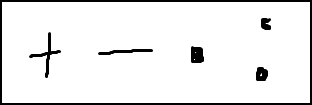
\includegraphics[height = 2cm]{graphics/data1.png} 
	\end{figure}	 
	
	Jeden taki plik zawiera 50 zestawów znaków umieszczonych w jednym wierszu. Łącznie baza danych składa się z 1200 znaków arytmetycznych, z czego 10\%  jest traktowana jako część walidacyjna. Za pomocą napisanego algorytmu, każdy plik jest dzielony na 200 osobnych obrazków, których piksele są zapisywane w dwuwymiarowej tablicy tak samo jak w przypadku bazy danych MNIST. Z racji tego, że możliwe są tylko cztery etykiety, dodawane są naprzemiennie, gdyż kolejność oznaczeń jest taka sama (plus, minus, mnożenie, dzielenie). Występują w tablicy jako wiersze zer z jedynką na jednym z czterech ostatnich indeksów. 
	
	\vspace{20 pt}
	Pozostałe pliki składają się z zestawów dziesięciu cyfr:
    \begin{figure}[h!]
	\centering
	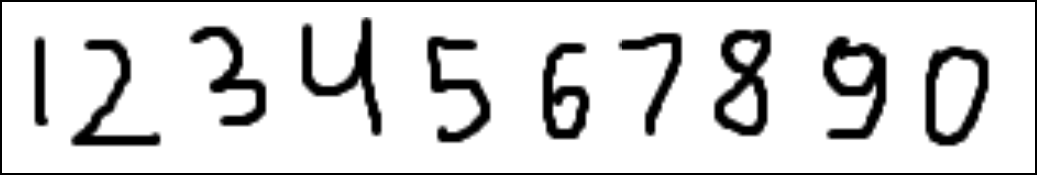
\includegraphics[height = 2cm]{graphics/data2.png} 
	\end{figure}
	
		W ich przypadku każdy z plików zawiera 15 zestawów umieszczonych w jednym wierszu. Łącznie baza danych składa się z 1200 cyfr, z czego 20\%  jest traktowana jako część walidacyjna. Tu ponownie wykorzystywany jest algorytm do dzielenia obrazu, a cyfry etykietowane są w postaci wierszy składających się z zer z jedną jeydnką na jednym z dziesięciu pierwszych indeksów.
		
\vspace{20pt} Baza ta w całości (2400 znaków) jest dołączona do wczytanej bazy MNIST, a następnie tasowana w celu zwiększenia efektywności nauczania.
	
\newpage	
\subsection*{Implementacja}
\subsubsection*{Informacje techniczne}
\hspace{20pt} Program został w całości napisany w języku C\# przy użyciu środowiska programistycznego Visual Studio z wykorzystaniem technologii WPF odpowiedzialnej za graficzny interfejs aplikacji.

\subsubsection*{Podział na pliki}
\hspace{20pt} Program został stworzony w dwóch wersjach. Pierwsza z nich, nazywana ,,Neural Network - Learning Place'', służy do uczenia sieci, zaś druga jest już właściwą aplikacją ,,Digit Recognizer''. W poniższym opisie skupiono się na wersji głównej. Projekt podzielony jest na 9 plików źródłowych:	
	\begin{itemize}
	\item Folder NeuralNetwork - w tym folderze znajdują się wszystkie pliki odpowiadające za działanie sieci neuronowej:
		\begin{itemize}
		\item Data.cs - plik zawierający wszystkie metody odpowiadające za przygotowanie danych i ich wczytywanie,
		\item Functions.cs - plik zawierający funkcje wykorzystywane przez neurony,
		\item Layer.cs - plik zawierający klasę symulującą warstwę sieci neuronowej,
		\item Network.cs - plik z główną klasą symulującą sieć neuronową,
		\item Neuron.cs - plik z klasą symulującą neuron,
		\item Synapse.cs - plik z klasą symulującą synapsę. 
		\end{itemize}
	\item Calculation.cs - plik z metodami odpowiedzialnymi za prawidłowe obliczenia; zawiera implementację Odwróconej Notacji Polskiej,
	\item DigitDetection.cs - plik zawierający przede wszystkim metody przetwarzające obraz ze ,,strefy rysowania''. 
	\item MainWindow.xaml.cs - plik zawierający graficzny interfejs aplikacji, implementację \\strefy rysowania wraz z metodą rysującą oraz inicjujący działanie sieci neuronowej.
	\end{itemize}		
\subsubsection*{Data.cs}
Metody:
\begin{itemize}
    \item \lstinline{public static double[][][] PrepareDatasets(int MNISTDatasetSizeDivider)} - 	metoda ta \\ odpowiedzialna jest za wczytanie baz danych i zwrócenia ich w postaci trójwymiarowej tablicy składającej się z czterech tablic wymiarowych. Są to kolejno: tablica danych wejściowych treningowych, tablica oczekiwanych danych wyjściowych treningowych, tablica danych wejściowych walidacyjnych i tablica oczekiwanych danych wyjściowych walidacyjnych. Na samym początku wczytane zostają pliki zawierające bazy danych. Ilość wczytywanych danych jest kontrolowana przez nas, ponieważ stwierdziliśmy, że wykorzystanie całej bazy MNIST nie jest konieczne do prawidłowego działania programu. W tym celu używany jest jedyny argument tej funkcji - \lstinline{MNISTDatasetSizeDivider}. Po wczytaniu danych są one dzielone na zestaw treningowy oraz walidacyjny, a następnie są tasowane za pomocą metody \lstinline{Shuffle()}.
    \item \lstinline{public static void LoadMNISTDataset(string imagesName, string labelsName, double[][] Images, double[][] Labels, int MNISTDatasetSizeDivider)} - metoda wczytująca fragment bazy danych MNIST. W celu wczytania pierwszych wartości, o których mowa w sekcji ,,Bazy danych'', korzysta z pomocniczej metody \lstinline{ReadBigInt32()}. Następnie wczytuje pozostałe liczby zawarte w plikach, konwertuje je na zmienne typu double i zapisuje w tablicy. Podobnie działa dla zapisanych w bazie etykiet.
	\item \lstinline{private static void LoadOwnDatasets(double[][] trainImages, double[][] trainLabels,} \newline \lstinline{double[][] testImages, double[][] testLabels, string[] arithmeticFilePaths, string[] digitFilePaths, int MNISTDatasetSizeDivider)} - metoda ta jest odpowiedzialna za prawidłowe wczytanie naszej autorskiej bazy danych. Metoda działa zarówno dla cyfr, jak i znaków. Dla każdego zdjęcia wywoływana jest metoda konwertująca dane na tablice zmiennych typu double. Z powodu powtarzalnej sekwencji ułożenia cyfr i znaków arytmetycznych w bazie danych przypisywanie etykiet jest oparte na prostym działaniu modulo. Metoda ta operuje na wcześniej podanych tablicach zawierających dane walidayjne jak i dane treningowe, ,,doklejając'' bazę autorską do wczytanej bazy MNIST, dlatego nie zwraca żadnych wartości.
    \item \lstinline{public static void Shuffle(double[][] arr1, double[][] arr2)} - metoda tasująca elementy dwóch podanych tablic: zawierającej zdjęcia i zawierającej etykiety. Działanie wymaga dwóch tablic, aby zapobiec sytuacji, w której etykieta jest przypisana złemu obrazkowi i na odwrót - elementy z obu struktur są tasowane równocześnie.
    \item \lstinline{public static double[][] BitmapToArray(Bitmap bitmap)} - metoda konwerująca bitmapę na tablicę dwuwymiarową. Każdemu pikselowi przypisywana jest wartość różnicy 255 oraz średniej arytmetycznej wartości RGB. Możliwa jest też pewna modyfikacja, zamieniająca wszystkie liczby dodatnie na liczbę 1. Na koniec zwracana jest tablica reprezentująca bitmapę (obraz).
    \item \lstinline{public static List<double[]> RemoveSecondDimensions(List<double[][]> digits)} - metoda konwertująca tablicę dwuwymiarową na tablicę jednowymiarową. Jest to niezbędne do prawidłowego działania sieci neuronowej, gdyż sieć przyjmuje dane jako tablice jednowymiarowe.
    \item \lstinline{public static class Extensions, public static int ReadBigInt32(this BinaryReader br)} - statyczna klasa zawierająca metodę odpowiadającą za prawidłowe wczytanie bazy MNIST. Bajty w bazie MNIST są zapisane w tzw. big-endian. Jest to forma zapisu, w której najbardziej znaczący bajt jest zapisany jako pierwszy. Jeśli więc pracujemy na procesorach Intela (które wykorzystują tzw. little-endian), musimy odwrócić bajty. Metoda ta sprawdza, czy jest potrzeba konwersji, a jeśli tak, to konwertuje big-endian na little-endian.
	\end{itemize}
	
Spośród powyższych metod tylko dwie są wykorzystywane w głównym projekcie: \\ \lstinline{BitmapToArray} oraz \lstinline{RemoveSecondDimensions}. Pozostałe są zaimplementowane jedynie w wersji ,,Learning Place''.

\subsubsection*{Functions.cs}
\hspace{20pt} Klasa ta zawiera wszystkie funkcje matematyczne wykorzystywane w programie przez sieć neuronową. Posiada właściwość \lstinline{public double Alpha} będącą współczynnikiem korekcji wykorzystywanym podczas liczenia wartości funkcji aktywacji oraz jej pochodnej; jest on ustawiony na 0.8. Klasa zawiera następujące metody:
    \begin{itemize}
        \item \lstinline{public static double InputSumFunction(List<Synapse> Inputs, double bias = 0)} - metoda zwracająca sumę wartości zwróconych przez synapsy wejściowe danego neuronu. Do końcowego wyniku dodawany jest również bias (domyślnie ustawiony na 0),
        \item \lstinline{public static double BipolarLinearFunction(double input)} - metoda zwracająca wartość funkcji aktywacji (funkcja bipolarna liniowa). Jako argument przyjmuje wartość zwróconą przez metodę \lstinline{InputSumFunction()},
        \item \lstinline{public static double BipolarDifferential(double input)} - metoda zwracająca wartość pochodnej funkcji aktywacji. Wykorzystywana jest w algorytmie wstecznej propagacji,
        \item \lstinline{public static double CalculateError(List<double> outputs, int row, double[][]} \\ \lstinline{expectedresults)} - metoda odpowiedzialna za wyznaczenie błędu średniokwadratowego na podstawie uzyskanego wektora wyjściowego i oczekiwanego wektora wyjściowego. Funkcja ta jest używana jedynie do celów testowych podczas trenowania.
    \end{itemize}
\subsubsection*{Neuron.cs}
\hspace{20pt} Klasa reprezentująca neuron sieci neuronowej. Jej polami/właściwościami są: lista synaps wchodzących (\lstinline{public List<Synapse> Inputs}), lista synaps wychodzących (\lstinline{public List<Synapse> Outputs}), wartość na wejściu (\lstinline{public double InputValue}) oraz wartość na wyjściu (\lstinline{public double OutputValue}). Zawiera następujące metody:
\begin{itemize}
    \item \lstinline{public Neuron()} - konstruktor klasy, który inicjuje puste listy synaps.
	\item \lstinline{public void AddOutputNeuron(Neuron outputneuron)} - metoda, która łączy neuron bieżący z innym za pomocą synapsy. Tworzona jest nowa synapsa, która następnie jest dodawana do listy synaps wychodzących bieżącego neuronu oraz do listy synaps wchodzących neuronu następnego.
	\item \lstinline{public void AddInputSynapse(double input)} - metoda, która dodaje synapsę wejściową do neuronu bez łączenia z innym neuronem. Występuje jedynie w wejściowej warstwie sieci. Podobnie jak pozostałe synapsy, jest dodawana do listy synaps wchodzących.
	\item \lstinline{public void CalculateOutput()} - metoda przypisująca właściwości \lstinline{InputValue} wynik funkcji \lstinline{InputSumFunction()} oraz właściwości \lstinline{OutputValue} wynik funkcji \lstinline{BipolarLinearFunction()}.
	\item \lstinline{public void PushValueOnInput(double input)} - metoda, która przypisuje podany argument zmiennej \lstinline{PushedData} synapsie wejściowej pierwszej warstwy. 
	\end{itemize}
\subsubsection*{Synapse.cs}
 \hspace{20pt} Klasa reprezentująca synapsę sieci neuronowej. Zawiera ona zmienną \lstinline{static readonly Random tmp} potrzebną do generowania liczby pseudolosowej, dwie zmienne klasy Neuron \\ (\lstinline{internal Neuron FromNeuron, ToNeuron}) reprezentujące, od którego do którego neuronu synapsa została połączona, a także właściwości \lstinline{public double Weight}, przechowującą wagę synapsy, oraz \lstinline{public double PushedData}, która przechowuje wartości podane synapsie (jeśli jest to pierwsza warstwa). Klasa zawiera następujące metody:
\begin{itemize}
    \item \lstinline{public Synapse(Neuron fromneuron, Neuron toneuron)} - konstruktor przyjmujący za argumenty dwa neurony, które mają zostać połączone daną synapsą. W konstruktorze zmiennym \lstinline{FromNeuron} i \lstinline{ToNeuron} przypisywane są wartości podane jako argumenty, a właściwości \lstinline{Weight} przypisywana jest wartość losowana przy użyciu zmiennej \lstinline{tmp}.
	\item \lstinline{public Synapse(Neuron toNeuron, double output)} - konstruktor, który przyjmuje za argument neuron oraz dane liczbowe); wykorzystywany przy pierwszej warstwie , z tego samego powodu waga jest ustawiona na wartość 1.
	\item \lstinline{public double GetOutput()} - metoda zwracająca wynik z danej synapsy. Metoda sprawdza, czy wyowałana została z pierwszej warstwy - jeśli tak, to zwraca niezmienione dane, jeśli nie, to zmienna \lstinline{OutputValue} ze zmiennej \lstinline{FromNeuron} jest mnożona razy wagę. 
	\end{itemize}
\subsubsection*{Layer.cs}
\hspace{20pt} Klasa ta definiuje warstwę zaimplementowanej sieci neuronowej. Jej jedynym polem/właściwością jest \lstinline{public List<Neuron> Neurons}, czyli lista neuronów wchodzących w skład warstwy. Klasa posiada następujące metody:
	\begin{itemize}
	    \item \lstinline{public Layer(int numberofneurons)} - konstruktor klasy, inicjuje on listę Neuronów, dodając do niej podaną jako argument liczbę neuronów, 
	    \item \lstinline{public void ConnectLayers(Layer outputlayer)} - metoda, która łączy wszystkie neurony w warstwie z innymi neuronami w innej warstwie poprzez wielokrotne wywołanie metody \lstinline{AddOutputNeuron} z klasy \lstinline{Neuron}.
	    \item \lstinline{public void CalculateOutputLayer()} - metoda wywołująca funkcję \lstinline{CalculateOutput()} z klasy \lstinline{Neuron} dla wszystkich neuronów z listy. 
	\end{itemize}
\subsubsection*{Network.cs}
\hspace{20pt} Klasa reprezentująca sieć neuronową. Klasa zawiera statyczną zmienną \lstinline{static readonly} \\ \lstinline{double LearningRate}, która reprezentuje wielkość kroku w każdej iteracji podczas osiągania minimum tzw. funkcji celu (ang. loss function) - jest wykorzystywana w algorytmie wstecznej propagacji. Jej wartość ustawiono na 0.05. Następna zmienna, \lstinline{static double SynapsesCount}, przechowuje informację o tym, ile synaps liczy cała sieć neuronowa. Lista \lstinline{internal List<La-} \\ \lstinline{yer> Layers} przechowuje wszystkie zdefiniowane warstwy sieci. Tablica dwuwymiarowa \lstinline{internal double[][] ExpectedResults} przechowuje etykiety. a \lstinline{double[][] ErrorFunctionChanges} przechowuje wartości zmiany funkcji błędu $\delta$ dla każdego neuronu w sieci. Zmienna \lstinline{LearningRate} oraz obie tablice występują jedynie w wersji ,,Learning Place''. Metody w klasie:
	
	\begin{itemize}
	    \item \lstinline{public Network(double alpha, int inputneuronscount, int[] hiddenlayerssizes, int} \\ \lstinline{outputneuronscount)} - konstruktor sieci neuronowej. Na samym początku sprawdzana jest poprawność podanych argumentów, które później przypisywane są do pól. Następnie za pomocą metod \lstinline{AddFirstLayer()} i \lstinline{AddNextLayer()} tworzone są wszystkie warstwy sieci.
	    \item \lstinline{private void AddFirstLayer(int inputneuronscount)} - prywatna metoda, która tworzy \\ pierwszą warstwę sieci neuronowej, zawierającą \lstinline{inputneuronscount} neuronów. Następnie za pomocą pętli do każdego neuronu w warstwie dodawana jest synapsa wejściowa z wartością 0 za pomocą funkcji \lstinline{AddInputSynapse()}, a sama warstwa jest dodawana do listy warstw sieci \lstinline{Layers}.
	    \item \lstinline{private void AddNextLayer(Layer newLayer)} - metoda łącząca ostatnią warstwę sieci z kolejną warstwą neuronów. Nowa warstwa jest dodawana do listy \lstinline{Layers}.
	    \item \lstinline{public void PushInputValues(double[] inputs)} - metoda przekazująca sieci neuronowej dane wejściowe. Metoda sprawdza, czy dane są poprawne tzn. czy wektor wejściowy ma taki sam rozmiar co pierwsza warstwa sieci, po czym umieszcza je w synapsach wejściowych neuronów pierwszej warstwy za pomocą funkcji \lstinline{PushValueOnInput()} klasy \lstinline{Neuron}.
	    \item \lstinline{public void  PushExpectedValues(double[][] expectedvalues)} - metoda przekazująca sieci neuronowej poprawne dane wyjściowe. Po sprawdzeniu poprawności danych, metoda przypisuje zmiennej prywatnej \lstinline{ExpectedResults} podany argument.
	    \item \lstinline{public List<double> GetOutput()} - metoda zwracająca uzyskane dane wyjściowe w postaci listy liczb typu \lstinline{double}. Po zainicjowaniu listy \lstinline{output} na każdej z warstw zostaje wykonana metoda \lstinline{CalculateOutputOnLayer()} z klasy \lstinline{Layer}, aktywująca neurony poszczególnych warstw w sposób sekwencyjny. Dzięki temu neurony na warstwie wyjściowej będą miały przypisaną aktualną wartość \lstinline{OutputValue}. Wartości każdego neuronu z tej warstwy zostają dodane do listy \lstinline{output}, po czym jest ona zwracana.
	    \item \lstinline{public void Train(double[][][] datasets, double epochscount, bool showinfo = false,} \\ \lstinline{bool breaking = false)} - metoda trenująca sieć neuronową, przyjmująca za argument m.in. zestaw 4 tablic dwuwymiarowych (treningowych i testowych). Po wywołaniu metody \lstinline{PushExpectedValues()} wykonywana jest \lstinline{epochscount} razy pętla odpowiadająca za właściwe trenowanie sieci. W każdej iteracji do sieci wysyłane są wszystkie treningowe wektory wejściowe, do zmiennej \lstinline{outputs} przypisywane są uzyskane dane wyjściowe, a następnie zostaje wywołana metoda \lstinline{ChangeWeights()}. Liczony jest też błąd średniokwadratowy przy użyciu funkcji \lstinline{CalculateMeanSquareError()}. Jest on wypisywany na ekranie tylko wtedy, gdy podany argument \lstinline{showinfo} ma ustawioną wartość \lstinline{true}. Ponadto istnieje dodatkowe zabezpieczenie, które sprawdza, czy występuje tzw. overfitting, czyli przeuczenie sieci. Jeśli metoda wykryje przeuczenie, to kończy swoje działanie. Zabezpieczenie to jest aktywne tylko wtedy, gdy podany argument \lstinline{breaking} ma ustawioną wartość \lstinline{true}. Po zakończeniu uczenia wagi każdej synapsy są zapisywane do pliku \lstinline{weights.txt} za pomocą metody \lstinline{SaveNetworkToFile()}.
	    \item \lstinline{private double CalculateMeanSquareError(double[][] inputs, double[][] expectedout-} \\ \lstinline{puts, bool showerror = false)} - metoda licząca i zwracająca średnią wartość błędu średniokwadratowego dla podanego zbioru testowego przy użyciu funkcji \lstinline{CalculateError()} z klasy \lstinline{Functions}. Błąd jest wypisywany (o ile zmienna \lstinline{showerror} ma wartość \lstinline{true}) z dokładnością do 5 miejsc po przecinku.
	    \item \lstinline{private void  ChangeWeights(List<double> outputs, int row)} - metoda modyfikująca wagi wszystkich synaps sieci neuronowej zgodnie z algorytmem wstecznej propagacji (opisanym w sekcji ,,Opis działania sieci neuronowej''). Po zaktualizowaniu tablicy \lstinline{ErrorFun-} \\ \lstinline{ctionChanges} przy użyciu metody \lstinline{CalculateErrorFunctionChanges()} dla każdej synapsy wejściowej każdego neuronu każdej warstwy (poza pierwszą) zaczynając od wyjściowej waga zostaje zmieniona zgodnie ze wzorem: $w^k_{ij} = w^k_{ij} + LearningRate \cdot 2 \cdot \delta^k_i \cdot y^{k-1}_j$.
	    \item \lstinline{private void CalculateErrorFunctionChanges(List<double> outputs, int row)} - metoda aktualizująca tablicę \lstinline{ErrorFunctionChanges}. Na początku uzupełniana jest kolumna odpowiadająca ostatniej warstwie sieci - przebiega to zgodnie ze wzorem $\delta_i^K = f'(s^K_i) \cdot (d^K_{i} - y^K_{i})$ - a następnie kolumny odpowiadające wszystkim warstwom ukrytym zaczynając od końca zgodnie ze wzorem: $\delta_i^k = f'(s^k_i) \sum_{j=1}^{N_{k+1}} \delta^{k+1}_j w^{k+1}_{ij}$.
	    \item \lstinline{private void SaveNetworkToFile(string path)} - prosta metoda zapisująca wagi synaps do pliku, którego ścieżkę podano jako argument. Kilka pętli przeskakuje przez wszystkie warstwy, neurony i synapsy, zapisując wagi do zainicjowanej wcześniej listy \lstinline{tmp}. Zapisywane są również ustawienia sieci takie jak zmienna \lstinline{alpha} i liczba neuronów w każdej warstwie - znajdują się one na samym początku listy. Następnie lista zapisywana jest do pliku.
	    \item \lstinline{public static Network  LoadNetworkFromFile(string path)} - metoda wczytująca sieć neuronową z pliku, którego ścieżkę podano jako argument. Metoda tworzy nową sieć neuronową, podając w konstruktorze dane wczytane z podanego pliku, a następnie pętle przechodzą przez wszystkie warstwy, neurony i synapsy, wczytując wagi. Metoda zwraca obiekt klasy \lstinline{Network}.
	    \item \lstinline{public void CalculatePrecision(double[][][] datasets, bool shownumbers = false)} - metoda sprawdzająca precyzję sieci neuronowej. Do sieci wprowadzane są testowe wektory wejściowe, a uzyskane wartości wyjściowe sprawdzane są z oczekiwanymi etykietami z wykorzystaniem pomocniczej metody \lstinline{Classify()}. Na końcu wyświetlany jest procent poprawnych odpowiedzi zaokrąglony do czterech miejsc po przecinku.
	    \item \lstinline{public void Classify(double[][] testingOutputs, List<double> trueOutputs)} - pomocnicza metoda wyświetlająca oczekiwane etykiety oraz dane wyjściowe zwrócone przez sieć neuronową.
	    \item \lstinline{private double  CountSynapse()} - metoda licząca i zwracająca liczbę synaps w sieci neuronowej.
	\end{itemize}
	
Wiele z powyższych metod jest wykorzystywanych jedynie w wersji ,,Learning Place'' - są to metody związane z uczeniem i klasyfikacją: \lstinline{Train, CalculateErrorFunctionChanges, ChangeWeights, CalculateMeanSquareError, CalculatePrecision, PushExpectedValues, Classify, SaveNetworkToFile}.
\subsubsection*{Calculation.cs}
\hspace{20pt} Klasa ta zawiera implementację ONP i jest używana jedynie w głównej wersji programu. Jej metody to:
	\begin{itemize}
	    \item \lstinline{public static string Calculate(string equation)} - metoda przyjmująca działanie zapisane w zmiennej tekstowej, konwertująca na zapis ONP i zwracająca wynik wyrażenia. Korzysta z trzech metod pomocniczych: \lstinline{toRPN()}, \lstinline{ConvertToStack()} oraz \lstinline{evalRPN()}. Na samym początku jednak sprawdzane jest, czy działanie jest poprawnie zapisane tzn. czy nie kończy i nie zaczyna się na znaku arytmetycznym i czy nie nastąpiło dzielenie przez zero.
	    \item \lstinline{public static string toRPN(string token)} - algorytm zmieniający zapis normalny na zapis w odwróconej notacji polskiej. Każde działanie jest zdefiniowane w słowniku i przypisana zostaje mu odpowiednia waga (dodawaniu i odejmowaniu - 1; mnożeniu i dzieleniu - 2). Następnie tworzona jest zmienna reprezentująca stos. Pętla przeskakuje po każdym znaku w zmiennej i próbuje ją przekonwertować na typ \lstinline{double}. Jeśli operacja powiedzie się, to znaczy, cyfra dodawana jest do zmiennej \lstinline{result}. Jeśli natomiast nastąpi błąd, znak arytmetyczny dodawany jest do stosu.
	    
	    \item \lstinline{public static Stack<string> ConvertToStack(string tokens)} - prosta metoda pomocnicza, która konwertuje typ \lstinline{string} na \lstinline{Stack}. Jest to potrzebne do prawidłowego i łatwego korzystania z innych metod tej klasy.
	    \item \lstinline{public static double evalRPN(Stack<string> tokens)} - metoda wyliczająca wynik z odwróconej notacji polskiej. Przyjmuje za argument stos, a zwraca typ \lstinline{double}. Metoda jest wykonywana rekurencyjnie, gdzie sprawdzane są kolejne znaki arytmetyczne i na tej zasadzie liczby są dodawane, odejmowane, dzielone lub mnożone.
	\end{itemize}
\subsubsection*{DigitDetection.cs}
	\begin{itemize}
	    \item \lstinline{private static List<int> ColumnSearch(Bitmap btm)} - metoda odpowiedzialna jest za przeszukiwanie bitmapy w osi X w poszukiwaniu kolumn, w których znajdują się znaki/cyfry. Wykrywanie zrealizowane jest za pomocą funkcji \lstinline{GetPixel()}, która zwraca wartości RGB pikseli. Dwie pętle przeszukują każdą kolumnę od góry do dołu. W przypadku, w którym zostanie wykryty piksel, który nie jest biały, dana kolumna zostaje dodana do listy. Funkcja zwraca listę zawierającą indeksy tych kolumn.
	    \item \lstinline{private static List<int> RowSearch(List<int> StartX, List<int> StopX, Bitmap btm, int digit)} - metoda ta działa podobnie do \lstinline{ColumnSearch()}, lecz skupia się na przeszukiwaniu wierszy w każdym z przedziałów kolumn, w których wykryto znaki. Wywoływana jest dla każdego przedziału z osobna i zwraca listę indeksów wierszy, w których znajduje się znak dla konkretnego przedziału.
	    \item \lstinline{private static List<double[][]> IntervalsCounting(List<int> columnsWithBlackPoints,} \\ \lstinline{Bitmap btm)} - metoda, która wyznacza punkty kluczowe dla wycinania cyfr i znaków, zwraca wartość zwracaną przez \lstinline{VericalCropping()}.
	    \item \lstinline{private static List<double[][]> VerticalCropping(List<int> StartX, List<int> StopX,} \\ \lstinline{List<int> StartY, List<int> StopY, Bitmap btm)} - metoda ta kopiuje obszary ograniczone przez obliczone wcześniej punkty kluczowe i, wywołując metody \lstinline{ResizeImage()} oraz \lstinline{TransformToSquare()}, finalnie zwraca listę tablic dwuwymiarowych typu \lstinline{double} odpowiadających wykrytym znakom.
	    \item \lstinline{ResizeImage(Image image)} - metoda skalująca obraz do wymiarów 28x28 pikseli w celu prawidłowego działania sieci neuronowej. Kwadratowy obraz znaku na końcu jest przetwarzany przez funkcję \lstinline{BitmapToArray()} z klasy \lstinline{Data} i zwracany w postaci tablicy dwuwymiarowej typu \lstinline{double}.
	    \item \lstinline{TransformToSquare(Bitmap bmpCrop, Bitmap btm)} - metoda generuje kwadratową płaszczyznę z białym tłem na podstawie wymiarów przesłanej bitmapy, a następnie umieszcza ją w jej centrum - płaszczyzna i bitmapa są nakładane na siebie. Metoda przewiduje dodatkowe warunki generowania płaszczyzny dla mnożenia oraz odejmowania i zwraca przetransformowane obrazy.
	    \item \lstinline{public static List<double[][]> DetectDigits(MemoryStream picture)} - główna metoda wywołująca całą sekwencję. Jej argumentem jest zapisany w pamięci obraz, zwraca listę cyfr w postaci tablic dwuwymiarowych. Metoda ta występuje jedynie w głównej wersji projektu i jest wykorzystywana do analizy ,,strefy rysowania''.
	    \item \lstinline{public static List<double[][]> DetectDigits(Bitmap picture)} - inny wariant powyższej metody. Tym razem argumentem jest bitmapa. Metoda ta jest wykorzystywana w wersji ,,Learning Place'' podczas przetwarzania graficznej bazy danych.
	    \item \lstinline{public static string RecognizeDigits(List<double[]> digits, Network network)} - metoda przepuszczająca przez podaną w argumencie sieć kolejne tablice przekonwertowanych obrazów i zwracająca uzyskany od sieci ciąg znaków w postaci zmiennej typu \lstinline{string}.
	\end{itemize}

	\subsubsection*{MainWindow.xaml.cs}
    \begin{itemize}
        \item \lstinline{private void CanvasMouseDown(object sender, MouseButtonEventArgs e)} - metoda śledząca pozycję myszy w czasie, kiedy lewy przycisk jest wciśnięty.
        \item \lstinline{private void CanvasMouseMove(object sender, MouseEventArgs e)} - metoda śledząca pozycję myszy w trakcie przesuwania i rysująca linię pomiędzy punktem początkowym - z momentu wywołania - a nowym - po przesunięciu. Pomiędzy tymi punktami rysowana jest linia, co w efekcie ciągłego wywoływania metody w trakcie przesuwania myszy daje linię wzdłuż toru ruchu kursora.
        \item \lstinline{private void LaunchNetworkButtonClick(object sender, RoutedEventArgs e)} - metoda wywoływana w trakcie naciśnięcia przycisku ,,Uruchom sieć neuronową''. Powoduje załadowanie parametrów sieci z pliku. Jeśli operacja ładowania wag nie powiedzie się, pozostałe dwa przyciski nadal będą nieaktywne.
        \item \lstinline{private void ClearButtonClick(object sender, RoutedEventArgs e)} - metoda wywoływana w trakcie naciśnięcia przycisku ,,Wyczyść''. Powoduje odświeżenie strefy rysowania i usunięcie istniejących na niej linii.
        \item \lstinline{private void CalculateButtonClick(object sender, RoutedEventArgs e)} - metoda wywoływana w trakcie naciśnięcia przycisku ,,Oblicz''. Powoduje wysłanie grafiki strefy rysowania do wycięcia oraz uruchamia klasyfikację. Otrzymany wynik wyświetlany jest w oknie aplikacji.
        \item \lstinline{private MemoryStream SaveCanvas(Canvas canvas)} - zapisuje grafikę ze strefy rysowania w pamięci RAM.
    \end{itemize}

\vspace{20pt}
\subsection*{Testy}
    \subsubsection*{Uczenie sieci}
    \hspace{20pt} Trenowanie sieci z wykorzystaniem bazy MNIST już od samego początku było bardzo efektywne, a dokładność zaimplementowanej sztucznej sieci neuronowej wynosiła powyżej 90\%. Mimo to skuteczność rozpoznawania cyfr pisanych w ,,strefie rysowania'' nie była wystarczająco wysoka, dlatego dodano bazę autorską i przetestowano kilka konfiguracji sieci. Przy wykorzystaniu 1\% bazy MNIST i ograniczonej bazie autorskiej uzyskano następujące wyniki:
    
\begin{center}
 \begin{tabular}{||c c c c c||} 
 \hline
 L. w. ukrytych & L. neuronów & LR & $\alpha$ & Błąd średniokwadratowy \\
 \hline\hline
 2 & 100 & 0.05 & 0.5 & 0.207 \\ 
 \hline
 2 & 100 & 0.05 & 0.75 & 0.186 \\ 
 \hline
\end{tabular}
\end{center}

W powyższej tabeli LR oznacza współczynnik nauczania wykorzystywany w algorytmie wstecznej propagacji, a $\alpha$ to współczynnik korekcji wykorzystywany w funkcji aktywacji w neuronach. Błąd średniokwadratowy jest liczony na podstawie wzoru $E_1 = \sum_{i=1}^{n}(d_{i} - y_{i})^{2}$, gdzie n to wymiar wektora wyjściowego / liczba neuronów wyjściowych, d to wartość oczekiwana, a y to wartość uzyskana (na i-tej pozycji wektora wyjściowego). W tabeli zapisano średnią błędu wszystkich elementów należących do zbioru testowego. 

Już po pierwszych dwóch testach zauważono, że wzrost współczynnika $\alpha$ działa pozytywnie na zmniejszenie się błędu średniokwadratowego, dlatego zdecydowano go zwiększyć do poziomu 0.8. Zdecydowano także zwiększyć wykorzystanie bazy MNIST do 2\%. Uzyskano następujące wyniki:

\begin{center}
 \begin{tabular}{||c c c c c||} 
 \hline
 L. w. ukrytych & L. neuronów & LR & $\alpha$ & Błąd średniokwadratowy \\
 \hline\hline
 2 & 100 & 0.05 & 0.8 & 0.198 \\ 
 \hline
 3 & 100 & 0.05 & 0.8 & 0.156 \\ 
 \hline
 4 & 100 & 0.05 & 0.8 & 0.143 \\ 
 \hline
\end{tabular}
\end{center}

Następnie zdecydowano się powiększyć dwukrotnie autorską bazę danych i ostateczne osiągi sztucznej sieci neuronowej wyniosły:

\begin{center}
 \begin{tabular}{||c c c c c||} 
 \hline
 L. w. ukrytych & L. neuronów & LR & $\alpha$ & Błąd średniokwadratowy \\
 \hline\hline
 4 & 100 & 0.05 & 0.8 & 0.12 \\ 
 \hline
\end{tabular}
\end{center}

Niewątpliwie sieć można by było uczynić bardziej dokładną szukając lepszej konfiguracji sieci, jednak zdecydowano, że dalsze modyfikacje będą dotyczyły sposobu zapisu liczb w tablicy dwuwymiarowej. Mianowicie obrazki przekonwertowane na tablice liczb zmiennoprzecinkowych typu double z przedziału 0-255 zostały zmienione na tablice zer i jedynek w taki sposób, że liczby poniżej 10 zmieniono na zera, a liczby większe lub równe 10 na jedynki. Modyfikacja ta wpłynęła pozytywnie na rozpoznawanie większości cyfr.
    \subsubsection*{Napotkane błędy i ich eliminacja}
    \begin{itemize}
        \item \textbf{Niepoprawne skalowanie dla znaku mnożenia} - program, wycinając znak w celu zmiany jego rozmiaru, wkleja go na wygenerowane pole zależne od dłuższej krawędzi wycinka. Metoda ta wymagała dołożenia osobnego warunku skalowania dla znaku ,,*'', gdyż użycie standardowego dla innych cyfr i znaków mnożnika 1.5, powodowało rozciągnięcie tego znaku na cały obszar, co uniemożliwiało jego poprawne rozpoznanie. W celu eliminacji błędu mnożnik dla znaków o rozmiarach mniejszych niż 10 procent wysokości pola rysowania ustawiono na wartość 8.
        \item \textbf{Wykrywanie przez program pojedynczych pikseli oderwanych od figury} - pojawianie się zagubionych pikseli wynikało z niedoskonałości linii powstałej w strefie rysowania. Program, wykrywając piksel, interpretował go jako znak mnożenia, co doprowadzało do wyświetlenia komunikatu o błędnym zapisie - dwa znaki obok siebie. Rozwiązaniem tego problemu okazało się zwiększenie minimalnego odstępu pomiędzy figurami z 1 do 3 pikseli.
    \end{itemize}
    \subsubsection*{Inne napotkane problemy aplikacji i optymalizacja działania}
    \begin{itemize}
        \item \textbf{Duże wykorzystanie pamięci przez bitmapy} - algorytm wycinający wykorzystuje bitmapy, które przesyłane są pomiędzy kolejnymi funkcjami programu. W celu zminimalizowania zużycia program zmniejszono wykorzystanie bitmap do minimum i są one generowane tylko w miejscach, gdzie jest to konieczne. Pozwala to uniknąć przepełniania pamięci w przypadku dużej ilości figur wprowadzonej do strefy rysowania.
        \item \textbf{Duża złożoność obliczeniowo-czasowa podczas uruchamiania sieci neuronowej} - początkowo wciśnięcie przycisku ,,Uruchom sieć neuronową'' skutkowało pobraniem całej bazy danych, zbudowaniem na jej podstawie sieci, wczytaniem wag z pliku i wyliczeniem dokładności - trwało to nawet kilkanaście sekund; zrezygnowano z tego pomysłu umieszczając w pierwszej linii pliku z wagami informację o budowie sieci, dzięki czemu bazy danych nie są już potrzebne aplikacji, a uruchamianie trwa ułamek sekundy.
    \end{itemize}
    \subsubsection*{Test aplikacji}
    \hspace{20pt} Przeprowadzone przez nas testy polegały na wprowadzeniu do programu w celu rozpoznania kolejno każdego z 14 znaków dwudziestokrotnie. Zestawy wprowadzane były na bieżąco do strefy rysowania, a następnie dane wyjściowe porównywano z danymi wejściowymi. Sprawdzana była w ten sposób zdolność identyfikacji wprowadzonej figury oraz poprawność obliczeniowa programu. Na następnej stronie znajduje się wykres poprawności rozpoznania dla cyfr i znaków.
    \newpage
    \begin{center}
    \begin{tikzpicture}[scale=0.9]
        \begin{axis}[
        	x tick label style={
        		/pgf/number format/1000 sep=},
        	title={Test poprawności rozpoznawania dla cyfr},
        	ylabel=Procent,
        	enlargelimits=0.05,
        	legend style={at={(0.5,-0.1)},
        	anchor=north,legend columns=-1},
        	ybar interval = 0.6,
        ]
        \addplot 
        	coordinates {(0,100) (1,100) (2,85) (3,90) (4,100) (5,95) (6,95) (7,95) (8,95) (9, 95) (10,15)};
        \end{axis}
    \end{tikzpicture}
    
    \vspace{20pt}
    
    \begin{tikzpicture}[scale=0.9]
      \begin{axis}[
      title={Test poprawności rozpoznawania dla znaków},
        ybar,
        enlargelimits=0.15,
        legend style={at={(0.5,-0.1)},
          anchor=north,legend columns=-1},
        ylabel=Procent,
        symbolic x coords={znak +,znak -,znak x,znak :, x},
        ybar interval = 0.6,
        ]
        \addplot coordinates {(znak +,90) (znak -,100) (znak x,95) (znak :,100) (x,15)};
      \end{axis}
    \end{tikzpicture}
    \end{center}	
	\hspace{20pt}Zdolność obliczeniowa aplikacji okazała się w stu procentach precyzyjna, a sama aplikacja odporna na błędy logiczne. Ponadto zdolność rozpoznawania znaków również okazała się bardzo precyzyjna (błędy zdarzały się sporadycznie).
	\newpage
\section*{Pełen kod aplikacji}
	\subsection*{Digit Recognizer}
	\subsubsection*{MainWindow.xaml - szata graficzna}
	\begin{lstlisting}
	<Window x:Class="DigitRecognizer.MainWindow"
        xmlns="http://schemas.microsoft.com/winfx/2006/xaml/presentation"
        xmlns:x="http://schemas.microsoft.com/winfx/2006/xaml"
        xmlns:d="http://schemas.microsoft.com/expression/blend/2008"
        xmlns:mc="http://schemas.openxmlformats.org/markup-compatibility/2006"
        mc:Ignorable="d"
        Title="Digit Recognizer" Height="435" Width="800" ResizeMode="NoResize" Background="LightSkyBlue">
    <Grid>
        <Grid.RowDefinitions>
            <RowDefinition Height="2*" />
            <RowDefinition Height="1*"/>
            <RowDefinition Height="1*"/>
        </Grid.RowDefinitions>

        <Canvas x:Name="PaintSurface" Grid.Row="0" MouseDown="CanvasMouseDown" MouseMove="CanvasMouseMove" Height="200" Width="800"
                    HorizontalAlignment="Stretch" VerticalAlignment="Stretch">
            <Canvas.Background>
                <SolidColorBrush Opacity="100" Color="White" />
            </Canvas.Background>
        </Canvas>

        <TextBlock x:Name="MathTextBox" Text="WPROWADZ DZIALANIE W STREFIE RYSOWANIA" FontSize="20" 
                   Margin="20" Height="30" TextAlignment="Center" Grid.Row="1" Background="White"/>

        <WrapPanel HorizontalAlignment="Center" Grid.Row="2">
            <Button x:Name="LaunchButton" Click="LaunchNetworkButtonClick" Content="Uruchom siec neuronowa" Width="160" Height="30" Margin="20" Background="White"/>
            <Button x:Name="ClearButton" Click="ClearButtonClick" Content="Wyczysc" Width="150" Height="30" Margin="20" 
                    IsEnabled="False" Background="White"/>
            <Button x:Name="CalculateButton" Click="CalculateButtonClick" Content="Oblicz" Width="150" Height="30" Margin="20" 
                    IsEnabled="False" Background="White"/>
        </WrapPanel>
    </Grid>
</Window>
	\end{lstlisting}

	\subsubsection*{MainWindow.xaml.cs - interfejs graficzny}
	\begin{lstlisting}
using System.IO;
using System.Windows;
using System.Windows.Controls;
using System.Windows.Input;
using System.Windows.Media;
using System.Windows.Media.Imaging;
using System.Windows.Shapes;
using System.Collections.Generic;
using NeuralNetwork;
//using System.Diagnostics;

namespace DigitRecognizer
{
    public partial class MainWindow : Window
    {
        Point CurrentPoint = new Point();
        Network network;

        public MainWindow()
        {
            InitializeComponent();
        }

        #region Rysowanie
        private void CanvasMouseDown(object sender, MouseButtonEventArgs e)
        {
            if (e.ButtonState == MouseButtonState.Pressed)
                CurrentPoint = e.GetPosition(this);
        }

        private void CanvasMouseMove(object sender, MouseEventArgs e)
        {
            if (e.LeftButton == MouseButtonState.Pressed)
            {
                Line line = new Line
                {
                    StrokeThickness = 4,
                    Stroke = SystemColors.WindowTextBrush,
                    X1 = CurrentPoint.X,
                    Y1 = CurrentPoint.Y,
                    X2 = e.GetPosition(this).X,
                    Y2 = e.GetPosition(this).Y
                };

                CurrentPoint = e.GetPosition(this);
                PaintSurface.Children.Add(line);
            }
        }
        #endregion



        #region Przyciski
        private void LaunchNetworkButtonClick(object sender, RoutedEventArgs e)
        {
            try
            {
                network = Network.LoadNetworkFromFile("weights.txt");
                LaunchButton.IsEnabled = false;
                CalculateButton.IsEnabled = true;
                ClearButton.IsEnabled = true;
                MathTextBox.Text = "SIEC GOTOWA!";
            }
            catch { MathTextBox.Text = "NIE ZNALEZIONO PRAWIDLOWEGO PLIKU Z WAGAMI!"; }
        }

        private void ClearButtonClick(object sender, RoutedEventArgs e)
        {
            PaintSurface.Children.Clear();
            MathTextBox.Text = "WPROWADZ NOWE DZIALANIE W STREFIE RYSOWANIA";
        }

        private void CalculateButtonClick(object sender, RoutedEventArgs e)
        {
            var picture = SaveCanvas(PaintSurface);      // Zapisuje canvas w pamieci
            var DigitsInTwoDimensions = DigitDetection.DetectDigits(picture); // Wywolanie kolejnych funkcji do wycinania i obrobki wczytanych cyfr, znakow

            List<double[]> digits = Data.RemoveSecondDimensions(DigitsInTwoDimensions); // Przygotowanie pod karmienie sieci 

            string tmp = DigitDetection.RecognizeDigits(digits, network);
            if (tmp != "") MathTextBox.Text = tmp;
            string result = Calculation.Calculate(tmp).ToString();
            if (result == "BLEDNY ZAPIS!" || result == "NIE MOZNA DZIELIC PRZEZ ZERO!") MathTextBox.Text = result;
            else MathTextBox.Text += result;
        }
        #endregion

        // Zapis Canvas:
        private MemoryStream SaveCanvas(Canvas canvas)
        {
            RenderTargetBitmap renderBitmap = new RenderTargetBitmap((int)canvas.Width, (int)canvas.Height, 96d, 96d, PixelFormats.Pbgra32);
            
            canvas.Measure(new Size((int)canvas.Width, (int)canvas.Height));
            canvas.Arrange(new Rect(new Size((int)canvas.Width, (int)canvas.Height)));
            renderBitmap.Render(canvas);
            JpegBitmapEncoder encoder = new JpegBitmapEncoder();
            encoder.Frames.Add(BitmapFrame.Create(renderBitmap));

            MemoryStream stream = new MemoryStream();
            encoder.Save(stream);

            return stream;
        }
    }
}
	\end{lstlisting}

\vspace{20pt}
	\subsubsection*{DigitDetection.cs - wyodrębnianie i obróbka liczb z obrazów}
	\begin{lstlisting}
using System.Collections.Generic;
using System.Drawing;
using System.Drawing.Drawing2D;
using System.Drawing.Imaging;
using System.IO;
using System.Linq;
using System.Diagnostics;
using NeuralNetwork;

namespace DigitRecognizer
{
    class DigitDetection
    {
        // Przeszukuje kolumny w celu znalezienia punktow innych niz biale:
        private static List<int> ColumnSearch(Bitmap btm)
        {
            List<int> Cols = new List<int>();
            Color color;
            for (int j = 0; j < btm.Width; j++)
                for (int i = 0; i < btm.Height; i++)
                {
                    color = btm.GetPixel(j, i);
                    if (color != Color.FromArgb(255, 255, 255))
                    {
                        Cols.Add(j);
                        break;
                    }
                }
            return Cols;
        }


        //Przeszukuje przedzialy znalezione przez ColumnSearch w poszukiwaniu punktow innych niz biale:
        private static List<int> RowSearch(List<int> StartX, List<int> StopX, Bitmap btm, int digit)
        {
            List<int> Rows = new List<int>();
            Color color;
            for (int k = 0; k < btm.Height; k++)
                for (int j = StartX[digit]; j < StopX[digit]; j++)
                {
                    color = btm.GetPixel(j, k);
                    if (color != Color.FromArgb(255, 255, 255))
                    {
                        Rows.Add(k);
                        break;
                    }
                }
            
            if (Rows.Count == 0) //Zabezpieczenie
            {
                Rows.Add(0);
                Rows.Add(btm.Height);
            }

            return Rows;
        }


        private static List<double[][]> IntervalsCounting(List<int> columnsWithBlackPoints, Bitmap btm)
        {
            if (columnsWithBlackPoints.Count == 0)
                return new List<double[][]>();

            //Przedzialy miedzy kolumnami
            List<int> StartX = new List<int>();
            List<int> StopX = new List<int>();

            StartX.Add(columnsWithBlackPoints[0]);
            for (int i = 1; i < columnsWithBlackPoints.Count - 1; i++)
                if (columnsWithBlackPoints[i + 1] - columnsWithBlackPoints[i] > 3)
                {
                    StartX.Add(columnsWithBlackPoints[i + 1]);
                    StopX.Add(columnsWithBlackPoints[i]);
                }
            StopX.Add(columnsWithBlackPoints[columnsWithBlackPoints.Count - 1]);


            //Przedzialy miedzy wierszami
            List<int> StartY = new List<int>();
            List<int> StopY = new List<int>();
            int digits = StartX.Count; //Tyle znaleziono znakow
            for (int i = 0; i < digits; i++)
            {
                List<int> Rows = RowSearch(StartX, StopX, btm, i); //Dla kazdego przedzialu kolumn z osobna
                if (Rows.Count != 0)
                {
                    StartY.Add(Rows[0]);
                    StopY.Add(Rows[Rows.Count - 1]);
                }
            }
            return VerticalCropping(StartX, StopX, StartY, StopY, btm);
        }

        // Dla obliczonych przedzialow wycinamy obrazy i wywolujemy funkcje skalujaca wyciete obrazy:
        private static List<double[][]> VerticalCropping(List<int> StartX, List<int> StopX, List<int> StartY, List<int> StopY, Bitmap btm)
        {
            int width, height;
            Bitmap bmpImage = new Bitmap(btm);
            List<double[][]> digits = new List<double[][]>();

            for (int i = 0; i < StartX.Count; i++)
            {
                width = StopX[i] - StartX[i];
                height = StopY[i] - StartY[i];
                if (width > 0 && height > 0)
                {
                    Bitmap bmpCrop = bmpImage.Clone(new Rectangle(StartX[i], StartY[i], width, height), bmpImage.PixelFormat);
                    digits.Add(ResizeImage(TransformToSquare(bmpCrop, btm)));
                }
            }
            return digits;
        }

        private static Bitmap TransformToSquare(Bitmap bmpCrop, Bitmap btm)
        { 
            int height, width;
            if(bmpCrop.Height < btm.Height*0.15 && bmpCrop.Width < btm.Height * 0.15) // "*"
            {
                height = (int)(bmpCrop.Height * 8);
                width = (int)(bmpCrop.Height * 8);
            }
            else if (bmpCrop.Height > bmpCrop.Width) // "-"
            {
                height = (int)(bmpCrop.Height * 1.5);
                width = (int)(bmpCrop.Height * 1.5);
            }
            else
            {
                height = (int)(bmpCrop.Width * 1.5);
                width = (int)(bmpCrop.Width * 1.5);
            }
            Bitmap bitmap = new Bitmap(width, height);
            using (var g = Graphics.FromImage(bitmap))
            {
                g.FillRectangle(Brushes.White, 0, 0, width, height);
                int x = width / 2 - bmpCrop.Width / 2;
                int y = height / 2 - bmpCrop.Height / 2;
                g.DrawImage(bmpCrop, x, y);
            }
            return bitmap;
        }


        // Funkcja zmieniajaca rozdzielczosc na 28x28 i zwracajaca bitmape w postaci tablicy dwuwymiarowej:
        private static double[][] ResizeImage(Image image)
        {
            int width = 28, height = 28;
            Rectangle croppSize = new Rectangle(0, 0, width, height);
            Bitmap resizedImage = new Bitmap(width, height);
            resizedImage.SetResolution(image.HorizontalResolution, image.VerticalResolution);

            using (var graphics = Graphics.FromImage(resizedImage))
            {
                graphics.CompositingMode = CompositingMode.SourceCopy;
                graphics.CompositingQuality = CompositingQuality.HighQuality;
                graphics.InterpolationMode = InterpolationMode.HighQualityBicubic;
                graphics.SmoothingMode = SmoothingMode.HighQuality;
                graphics.PixelOffsetMode = PixelOffsetMode.HighQuality;

                using (var wrapMode = new ImageAttributes())
                {
                    wrapMode.SetWrapMode(WrapMode.TileFlipXY);
                    graphics.DrawImage(image, croppSize, 0, 0, image.Width, image.Height, GraphicsUnit.Pixel, wrapMode);
                }
            }
            return Data.BitmapToArray(resizedImage);
        }

        // Glowna funkcja wywolujaca sekwencje:
        public static List<double[][]> DetectDigits(MemoryStream picture)
        {
            Bitmap btm = new Bitmap(picture);
            return IntervalsCounting(ColumnSearch(btm), btm);  // Analiza dzialania, wyciecie i zapis
        }

        public static string RecognizeDigits(List<double[]> digits, Network network)
        {
            string tmp = "";
            foreach (double[] digit in digits)
            {
                network.PushInputValues(digit);
                var output = network.GetOutput();

                for (int i = 0; i < output.Count; i++)
                    Debug.WriteLine(output[i] + " ");
                Debug.WriteLine("");

                
                double max = output.Max();
                //if (max < 0.5) return $"NIE POTRAFIE ROZPOZNAC {digits.IndexOf(digit) + 1}. ZNAKU";

                //int count = 0; 
                //foreach (double i in output) if (i > 0.7) count++;
                //if (count > 1) return $"NIE POTRAFIE ROZPOZNAC {digits.IndexOf(digit) + 1}. ZNAKU";

                string[] signs = { "0", "1", "2", "3", "4", "5", "6", "7", "8", "9", "+", "-", "*", "/" };
                int index = output.IndexOf(max);
                if (index >= 10) tmp += " " + signs[index] + " ";
                else tmp += signs[index];
            }
            return tmp;
        }
    }
}
	\end{lstlisting}

\vspace{20pt}	
	\subsubsection*{Calculation.cs - funkcje wyliczeniowe}
	\begin{lstlisting}
using System;
using System.Collections.Generic;

namespace DigitRecognizer
{
    class Calculation
    {
        public static string Calculate(string equation)
        {
            if (equation.EndsWith(" - ") || equation.EndsWith(" + ") || equation.EndsWith(" * ") || equation.EndsWith(" / ") || equation.Contains("  "))
                return "BLEDNY ZAPIS!";
            if (equation.StartsWith(" - ") || equation.StartsWith(" + ") || equation.StartsWith(" * ") || equation.StartsWith(" / "))
                return "BLEDNY ZAPIS!";
            if (equation.Contains(" / 0")) return "NIE MOZNA DZIELIC PRZEZ ZERO!";
            Stack<string> temp = ConvertToStack(toRPN(equation));
            return " = " + evalRPN(temp).ToString();
        }

        public static string toRPN(string token) //metoda zwracajaca wyrazenie w RPN w stringu
        {
            Dictionary<string, int> precedence = new Dictionary<string, int>
            {
                { "+", 1 }, { "-", 1 }, { "/", 2 }, { "*", 2 }
            };

            Stack<string> stack = new Stack<string>();

            string result = "";
            string[] equation = token.Split(' ');

            foreach (string item in equation)
            {
                try
                {
                    double temp = Convert.ToDouble(item);
                    result += " " + item;
                }
                catch
                {
                    while (stack.Count != 0 && precedence[item] <= precedence[stack.Peek()])
                        result += " " + stack.Pop();

                    stack.Push(item);
                }
            }

            while (stack.Count != 0)
                result += " " + stack.Pop();

            result = result.Remove(0, 1);

            return result;
        }

        public static Stack<string> ConvertToStack(string tokens) //metoda konwertujaca string na Stack
        {
            string[] result = tokens.Split();
            Stack<string> stack = new Stack<string>();

            foreach (string token in result)
                stack.Push(token);

            return stack;
        }

        public static double evalRPN(Stack<string> tokens) //metoda zwracajaca wynik wyrazenia w RPN
        { 
            string token = tokens.Pop();
            double firstNumber, secondNumber;

            if (!Double.TryParse(token, out firstNumber))
            {
                secondNumber = evalRPN(tokens);
                firstNumber = evalRPN(tokens);

                if (token == "+")
                    firstNumber += secondNumber;
                else if (token == "-")
                    firstNumber -= secondNumber;
                else if (token == "*")
                    firstNumber *= secondNumber;
                else if (token == "/")
                    firstNumber /= secondNumber;
                else throw new Exception();
            }

            return firstNumber;
        }
    }
}
	\end{lstlisting}
	
	\vspace{20pt}	
	\subsubsection*{NeuralNetwork/Data.cs}
	\begin{lstlisting}
using System.Collections.Generic;
using System.Drawing;

namespace NeuralNetwork
{
   class Data
    {
        public static double[][] BitmapToArray(Bitmap bitmap)
        {
            double[][] values = new double[bitmap.Height][];
            for (int i = 0; i < values.Length; i++)
                values[i] = new double[bitmap.Width];

            for (int i = 0; i < bitmap.Height; i++)
                for (int j = 0; j < bitmap.Width; j++)
                {
                    values[i][j] = 255 - (bitmap.GetPixel(j, i).R + bitmap.GetPixel(j, i).G + bitmap.GetPixel(j, i).B) / 3;
                    //if (values[i][j] >= 10) values[i][j] = 1;
                    //else values[i][j] = 0;
                }

            return values;
        }

        public static List<double[]> RemoveSecondDimensions(List<double[][]> digits)
        {
            List<double[]> tmp = new List<double[]>();
            foreach (double[][] digit in digits)
            {
                List<double> newlist = new List<double>();
                for (int i = 0; i < digit.Length; i++)
                    for (int j = 0; j < digit[i].Length; j++)
                        newlist.Add(digit[i][j]);

                tmp.Add(newlist.ToArray());
            }
            return tmp;
        }
    }
}
	\end{lstlisting}
	
	\vspace{20pt}	
	\subsubsection*{NeuralNetwork/Network.cs}
	\begin{lstlisting}
using System;
using System.Collections.Generic;
using System.IO;

namespace NeuralNetwork
{
    class Network
    {
        static double SynapsesCount;
        internal List<Layer> Layers;

        public Network(double alpha, int inputneuronscount, int[] hiddenlayerssizes, int outputneuronscount)
        {
            if (inputneuronscount < 1 || hiddenlayerssizes.Length < 1 || outputneuronscount < 1)
                throw new Exception("Incorrect Network Parameters");

            Functions.Alpha = alpha;

            Layers = new List<Layer>();
            AddFirstLayer(inputneuronscount);
            for (int i = 0; i < hiddenlayerssizes.Length; i++)
                AddNextLayer(new Layer(hiddenlayerssizes[i]));
            AddNextLayer(new Layer(outputneuronscount));

            SynapsesCount = CountSynapses();
        }

        private void AddFirstLayer(int inputneuronscount)
        {
            Layer inputlayer = new Layer(inputneuronscount);
            foreach (Neuron neuron in inputlayer.Neurons) 
                neuron.AddInputSynapse(0);
            Layers.Add(inputlayer);
        }

        private void AddNextLayer(Layer newlayer)
        {
            Layer lastlayer = Layers[Layers.Count - 1];
            lastlayer.ConnectLayers(newlayer);
            Layers.Add(newlayer);
        }

        public void PushInputValues(double[] inputs)
        {
            if (inputs.Length != Layers[0].Neurons.Count) 
                throw new Exception("Incorrect Input Size");

            for (int i = 0; i < inputs.Length; i++) 
                Layers[0].Neurons[i].PushValueOnInput(inputs[i]);
        }

        public List<double> GetOutput()
        {
            List<double> output = new List<double>();
            for (int i = 0; i < Layers.Count; i++)
                Layers[i].CalculateOutputOnLayer();
            foreach (Neuron neuron in Layers[Layers.Count - 1].Neurons)
                output.Add(neuron.OutputValue);
            return output;
        }

        public static Network LoadNetworkFromFile(string path)
        {
            string[] lines = File.ReadAllLines(path);
            string[] firstLine = lines[0].Split();
            List<int> hiddenLayerSizes = new List<int>();
            for (int i = 2; i < firstLine.Length - 1; i++)
                hiddenLayerSizes.Add(Convert.ToInt32(firstLine[i]));

            Network net = new Network(double.Parse(firstLine[0]), Convert.ToInt32(firstLine[1]),
                hiddenLayerSizes.ToArray(), Convert.ToInt32(firstLine[firstLine.Length - 1]));

            if (lines.Length - 1 != SynapsesCount)
                throw new Exception("Incorrect Input File");
            else
            {
                try
                {
                    int i = 1;
                    for (int j = 1; j < net.Layers.Count; j++)
                        foreach (Neuron neuron in net.Layers[j].Neurons)
                            foreach (Synapse synapse in neuron.Inputs)
                                synapse.Weight = double.Parse(lines[i++]);
                }
                catch (Exception) { throw new Exception("Incorrect Input File"); }
            }
            return net;
        }

        private double CountSynapses()
        {
            double count = 0;
            for (int i = 1; i < Layers.Count; i++)
                foreach (Neuron neuron in Layers[i].Neurons)
                    foreach (Synapse synapse in neuron.Inputs)
                        count++;
            return count;
        }
    }
}
	\end{lstlisting}
	
	\vspace{20pt}	
	\subsubsection*{NeuralNetwork/Layer.cs}
	\begin{lstlisting}
using System.Collections.Generic;

namespace NeuralNetwork
{
    class Layer
    {
        public List<Neuron> Neurons;

        public Layer(int numberofneurons)
        {
            Neurons = new List<Neuron>();
            for (int i = 0; i < numberofneurons; i++)
                Neurons.Add(new Neuron());
        }

        public void ConnectLayers(Layer outputlayer)
        {
            foreach (Neuron thisneuron in Neurons)
                foreach (Neuron thatneuron in outputlayer.Neurons)
                    thisneuron.AddOutputNeuron(thatneuron);
        }

        public void CalculateOutputOnLayer()
        {
            foreach (Neuron neuron in Neurons) 
                neuron.CalculateOutput();
        }
    }
}
	\end{lstlisting}
	
	\vspace{20pt}	
	\subsubsection*{NeuralNetwork/Neuron.cs}
	\begin{lstlisting}
using System.Collections.Generic;

namespace NeuralNetwork
{
    class Neuron
    {
        public List<Synapse> Inputs { get; set; }
        public List<Synapse> Outputs { get; set; }
        public double InputValue { get; set; }
        public double OutputValue { get; set; }

        public Neuron()
        {
            Inputs = new List<Synapse>();
            Outputs = new List<Synapse>();
        }

        public void AddOutputNeuron(Neuron outputneuron)
        {
            Synapse synapse = new Synapse(this, outputneuron);
            Outputs.Add(synapse); outputneuron.Inputs.Add(synapse);
        }

        public void AddInputSynapse(double input)
        {
            Synapse syn = new Synapse(this, input);
            Inputs.Add(syn);
        }

        public void CalculateOutput()
        {
            InputValue = Functions.InputSumFunction(Inputs);
            OutputValue = Functions.BipolarLinearFunction(InputValue);
        }

        public void PushValueOnInput(double input) 
        { 
            Inputs[0].PushedData = input; 
        }
    }
}
	\end{lstlisting}
	
	\vspace{20pt}	
	\subsubsection*{NeuralNetwork/Synapse.cs}
	\begin{lstlisting}
using System;

namespace NeuralNetwork
{
    class Synapse
    {
        static readonly Random tmp = new Random();
        internal Neuron FromNeuron, ToNeuron;
        public double Weight { get; set; }
        public double PushedData { get; set; }

        public Synapse(Neuron fromneuron, Neuron toneuron) // zwykla synapsa
        {
            FromNeuron = fromneuron; ToNeuron = toneuron;
            Weight = tmp.NextDouble() - 0.5;
        }

        public Synapse(Neuron toneuron, double output)     // synapsa wejsciowa pierwszej warstwy
        {
            ToNeuron = toneuron; PushedData = output; 
            Weight = 1;
        }

        public double GetOutput()
        {
            if (FromNeuron == null) return PushedData;
            return FromNeuron.OutputValue * Weight;
        }
    }
}
	\end{lstlisting}
	\vspace{20pt}	
	\subsubsection*{NeuralNetwork/Functions.cs}
	\begin{lstlisting}
using System;
using System.Collections.Generic;

namespace NeuralNetwork
{
    class Functions
    {
        public static double Alpha { get; set; } = 0.8;

        public static double InputSumFunction(List<Synapse> Inputs) 
            // funkcja wejscia: suma iloczynow wag synaps wchodzacych i wartosci wyjsciowych neuronow warstwy poprzedniej
        {
            double input = 0;
            foreach (Synapse syn in Inputs) 
                input += syn.GetOutput();
            return input;
        }

        public static double BipolarLinearFunction(double input) // funkcja aktywacji: bipolarna liniowa
            => (1 - Math.Pow(Math.E, -Alpha * input)) / (1 + Math.Pow(Math.E, -Alpha * input));
    }
}
	\end{lstlisting}

\vspace{20pt}
    \subsection*{Neural Network - Learning Place}
	\subsubsection*{Data.cs}
	\begin{lstlisting}
using System;
using System.IO;
using System.Collections.Generic;
using System.Drawing;

namespace NeuralNetwork
{
    class Data
    {
        public static double[][][] PrepareDatasets(int MNISTDatasetSizeDivider)
        {
            Console.WriteLine(" Loading datasets...");
            string[] arithmeticFilePaths = Directory.GetFiles(@"Datasets\", "signs*.png");
            string[] digitFilePaths      = Directory.GetFiles(@"Datasets\", "digits*.png");
            double[][] trainImages = new double[60000 / MNISTDatasetSizeDivider + arithmeticFilePaths.Length * 180 + digitFilePaths.Length * 120][];
            double[][] trainLabels = new double[60000 / MNISTDatasetSizeDivider + arithmeticFilePaths.Length * 180 + digitFilePaths.Length * 120][];
            for (int i = 0; i < trainImages.Length; i++)
                trainImages[i] = new double[28 * 28];
            for (int i = 0; i < trainLabels.Length; i++)
                trainLabels[i] = new double[14];

            double[][] testImages = new double[10000 / MNISTDatasetSizeDivider + arithmeticFilePaths.Length * 20 + digitFilePaths.Length * 30][];
            double[][] testLabels = new double[10000 / MNISTDatasetSizeDivider + arithmeticFilePaths.Length * 20 + digitFilePaths.Length * 30][];
            for (int i = 0; i < testImages.Length; i++)
                testImages[i] = new double[28 * 28];
            for (int i = 0; i < testLabels.Length; i++)
                testLabels[i] = new double[14];

            LoadMNISTDataset(@"Datasets\train-images.idx3-ubyte", @"Datasets\train-labels.idx1-ubyte", trainImages, trainLabels, MNISTDatasetSizeDivider);
            LoadMNISTDataset(@"Datasets\t10k-images.idx3-ubyte", @"Datasets\t10k-labels.idx1-ubyte", testImages, testLabels, MNISTDatasetSizeDivider);
            LoadOwnDatasets(trainImages, trainLabels, testImages, testLabels, arithmeticFilePaths, digitFilePaths, MNISTDatasetSizeDivider);
            Shuffle(trainImages, trainLabels);

            return new double[][][] { trainImages, trainLabels, testImages, testLabels };
        }

        private static void LoadOwnDatasets(double[][] trainImages, double[][] trainLabels, 
            double[][] testImages, double[][] testLabels, string[] arithmeticFilePaths, string[] digitFilePaths, int MNISTDatasetSizeDivider)
        {
            int trainIndex = 60000 / MNISTDatasetSizeDivider, testIndex = 10000 / MNISTDatasetSizeDivider;

            // Znaki arytmetyczne:
            List<double[]> arithmeticSigns; int tempIndex = 0;
            for (int i = 0; i < arithmeticFilePaths.Length; i++)
            {
                arithmeticSigns = RemoveSecondDimensions(DigitDetection.DetectDigits(new Bitmap(arithmeticFilePaths[i])));
                for (int j = 0; j < arithmeticSigns.Count - 20; j++)
                {
                    trainImages[trainIndex] = arithmeticSigns[j];
                    for (int k = 0; k < trainImages[trainIndex].Length; k++)
                    {
                        if (trainImages[trainIndex][k] < 10) trainImages[trainIndex][k] = 0;
                        else trainImages[trainIndex][k] = 1;
                    }
                    trainLabels[trainIndex][(tempIndex++ % 4) + 10] = 1;
                    trainIndex++;
                }
                for (int j = arithmeticSigns.Count - 20; j < arithmeticSigns.Count; j++) // ostatnie 20 znakow (czyli 10%, bo mamy pliki po 200 znakow) idzie do testowego
                {
                    testImages[testIndex] = arithmeticSigns[j];
                    for (int k = 0; k < testImages[testIndex].Length; k++)
                    {
                        if (testImages[testIndex][k] < 10) testImages[testIndex][k] = 0;
                        else testImages[testIndex][k] = 1;
                    }
                    testLabels[testIndex][(tempIndex++ % 4) + 10] = 1;
                    testIndex++;
                }
            }

            // Cyfry:
            List<double[]> digits; tempIndex = 0;
            for (int i = 0; i < digitFilePaths.Length; i++)
            {
                digits = RemoveSecondDimensions(DigitDetection.DetectDigits(new Bitmap(digitFilePaths[i])));
                for (int j = 0; j < digits.Count - 30; j++)
                {
                    trainImages[trainIndex] = digits[j];
                    for(int k = 0; k < trainImages[trainIndex].Length; k++)
                    {
                        if (trainImages[trainIndex][k] < 10) trainImages[trainIndex][k] = 0;
                        else trainImages[trainIndex][k] = 1;
                    }
                    trainLabels[trainIndex][(tempIndex++ + 1) % 10] = 1;
                    trainIndex++;
                }
                for (int j = digits.Count - 30; j < digits.Count; j++) // ostatnie 30 znakow (czyli 20%, bo mamy pliki po 150 znakow) idzie do testowego
                {
                    testImages[testIndex] = digits[j];
                    for (int k = 0; k < testImages[testIndex].Length; k++)
                    {
                        if (testImages[testIndex][k] < 10) testImages[testIndex][k] = 0;
                        else testImages[testIndex][k] = 1;
                    }
                    testLabels[testIndex][(tempIndex++ + 1) % 10] = 1;
                    testIndex++;
                }
            }
        }

        private static void Shuffle(double[][] arr1, double[][] arr2)
        {
            Random rand = new Random();
            int j = arr1.Length;

            while(j > 1)
            {
                int k = rand.Next(j--);
                var temp1 = arr1[j];
                var temp2 = arr2[j];

                arr1[j] = arr1[k];
                arr1[k] = temp1;

                arr2[j] = arr2[k];
                arr2[k] = temp2;
            }
        }

        public static double[][] BitmapToArray(Bitmap bitmap)
        {
            double[][] values = new double[bitmap.Height][];
            for (int i = 0; i < values.Length; i++)
                values[i] = new double[bitmap.Width];

            for (int i = 0; i < bitmap.Height; i++)
                for (int j = 0; j < bitmap.Width; j++)
                    values[i][j] = 255 - (bitmap.GetPixel(j, i).R + bitmap.GetPixel(j, i).G + bitmap.GetPixel(j, i).B) / 3;

            return values;
        }

        private static void LoadMNISTDataset(string imagesName, string labelsName, double[][] Images, double[][] Labels, int MNISTDatasetSizeDivider)
        {
            BinaryReader brImages = new BinaryReader(new FileStream(imagesName, FileMode.Open));
            BinaryReader brLabels = new BinaryReader(new FileStream(labelsName, FileMode.Open));

            Extensions.ReadBigInt32(brImages);  // magic1
            int numImages = Extensions.ReadBigInt32(brImages);
            int numRows = Extensions.ReadBigInt32(brImages);
            int numCols = Extensions.ReadBigInt32(brImages);

            Extensions.ReadBigInt32(brLabels);  // magic2
            Extensions.ReadBigInt32(brLabels);  // numLabels

            for (int i = 0; i < numImages / MNISTDatasetSizeDivider; i++)
            {
                for (int j = 0; j < numRows * numCols; j++)
                {
                    Images[i][j] = Convert.ToDouble(brImages.ReadByte());
                    if (Images[i][j] < 10) Images[i][j] = 0;
                    else Images[i][j] = 1;
                }

                Labels[i][Convert.ToInt32(brLabels.ReadByte())] = 1;
            }
        }

        private static List<double[]> RemoveSecondDimensions(List<double[][]> digits)
        {
            List<double[]> tmp = new List<double[]>();
            foreach (double[][] digit in digits)
            {
                List<double> newlist = new List<double>();
                for (int i = 0; i < digit.Length; i++)
                    for (int j = 0; j < digit[i].Length; j++)
                        newlist.Add(digit[i][j]);

                tmp.Add(newlist.ToArray());
            }
            return tmp;
        }
    }

    public static class Extensions
    {
        public static int ReadBigInt32(this BinaryReader br)
        {
            var bytes = br.ReadBytes(sizeof(Int32));
            if (BitConverter.IsLittleEndian)
                Array.Reverse(bytes);
            return BitConverter.ToInt32(bytes, 0);
        }
    }
}
	\end{lstlisting}
	
	\vspace{20pt}	
	\subsubsection*{Network.cs}
	\begin{lstlisting}
using System;
using System.Collections.Generic;
using System.IO;
using System.Linq;

namespace NeuralNetwork
{
    class Network
    {
        static readonly double LearningRate = 0.05;
        static double SynapsesCount;
        internal List<Layer> Layers;
        internal double[][] ExpectedResults;
        double[][] ErrorFunctionChanges;

        public Network(double alpha, int inputneuronscount, int[] hiddenlayerssizes, int outputneuronscount)
        {
            Console.WriteLine(" Building neural network...");
            if (inputneuronscount < 1 || hiddenlayerssizes.Length < 1 || outputneuronscount < 1)
                throw new Exception("Incorrect Network Parameters");

            Functions.Alpha = alpha;

            Layers = new List<Layer>();
            AddFirstLayer(inputneuronscount);
            for (int i = 0; i < hiddenlayerssizes.Length; i++)
                AddNextLayer(new Layer(hiddenlayerssizes[i]));
            AddNextLayer(new Layer(outputneuronscount));

            SynapsesCount = CountSynapses();

            ErrorFunctionChanges = new double[Layers.Count][];
            for (int i = 1; i < Layers.Count; i++) 
                ErrorFunctionChanges[i] = new double[Layers[i].Neurons.Count];
        }

        private void AddFirstLayer(int inputneuronscount)
        {
            Layer inputlayer = new Layer(inputneuronscount);
            foreach (Neuron neuron in inputlayer.Neurons) 
                neuron.AddInputSynapse(0);
            Layers.Add(inputlayer);
        }

        private void AddNextLayer(Layer newlayer)
        {
            Layer lastlayer = Layers[Layers.Count - 1];
            lastlayer.ConnectLayers(newlayer);
            Layers.Add(newlayer);
        }

        public void PushInputValues(double[] inputs)
        {
            if (inputs.Length != Layers[0].Neurons.Count) 
                throw new Exception("Incorrect Input Size");

            for (int i = 0; i < inputs.Length; i++) 
                Layers[0].Neurons[i].PushValueOnInput(inputs[i]);
        }

        public void PushExpectedValues(double[][] expectedvalues) 
        {
            if (expectedvalues[0].Length != Layers[Layers.Count - 1].Neurons.Count) 
                throw new Exception("Incorrect Expected Output Size");

            ExpectedResults = expectedvalues;
        }

        public List<double> GetOutput()
        {
            List<double> output = new List<double>();
            for (int i = 0; i < Layers.Count; i++)
                Layers[i].CalculateOutputOnLayer();
            foreach (Neuron neuron in Layers[Layers.Count - 1].Neurons)
                output.Add(neuron.OutputValue);
            return output;
        }

        public void Train(double[][][] datasets, double epochscount, bool showinfo = false, bool breaking = false)
        {
            double[][] trainingInputs = datasets[0], trainingOutputs = datasets[1];
            double recenterror = double.MaxValue, minerror = double.MaxValue;

            PushExpectedValues(trainingOutputs);
            Console.WriteLine(" Training neural network...");
            for (int i = 0; i < epochscount; i++)
            {
                List<double> outputs = new List<double>();
                for (int j = 0; j < trainingInputs.Length; j++)
                {
                    PushInputValues(trainingInputs[j]);
                    outputs = GetOutput();
                    ChangeWeights(outputs, j);
                }

                recenterror = CalculateMeanSquareError(datasets[2], datasets[3], showinfo);
                if (breaking == true && minerror < recenterror) break;
                minerror = recenterror;
            }

            SaveNetworkToFile("weights.txt");
            Console.WriteLine(" Done!");
        }

        private double CalculateMeanSquareError(double[][] inputs, double[][] expectedoutputs, bool showerror = false)
        {
            double error = 0; 
            List<double> outputs = new List<double>();
            for (int i = 0; i < inputs.Length; i++)
            {
                PushInputValues(inputs[i]);
                outputs = GetOutput();
                error += Functions.CalculateError(outputs, i, expectedoutputs);
            }
            error /= inputs.Length;
            if (showerror == true) Console.WriteLine($" Average mean square error: {Math.Round(error, 5)}");
            return error;
        }

        private void ChangeWeights(List<double> outputs, int row) // przy uzyciu algorytmu wstecznej propagacji
        {
            CalculateErrorFunctionChanges(outputs, row);
            for (int k = Layers.Count - 1; k > 0; k--)
                for (int i = 0; i < Layers[k].Neurons.Count; i++)
                    for (int j = 0; j < Layers[k - 1].Neurons.Count; j++)
                        Layers[k].Neurons[i].Inputs[j].Weight += 
                            LearningRate * 2 * ErrorFunctionChanges[k][i] * Layers[k - 1].Neurons[j].OutputValue;
        }

        private void CalculateErrorFunctionChanges(List<double> outputs, int row)
        {
            for (int i = 0; i < Layers[Layers.Count - 1].Neurons.Count; i++)
                ErrorFunctionChanges[Layers.Count - 1][i] = (ExpectedResults[row][i] - outputs[i])
                    * Functions.BipolarDifferential(Layers[Layers.Count - 1].Neurons[i].InputValue);
            for (int k = Layers.Count - 2; k > 0; k--)
                for (int i = 0; i < Layers[k].Neurons.Count; i++)
                {
                    ErrorFunctionChanges[k][i] = 0;
                    for (int j = 0; j < Layers[k + 1].Neurons.Count; j++)
                        ErrorFunctionChanges[k][i] += ErrorFunctionChanges[k + 1][j] * Layers[k + 1].Neurons[j].Inputs[i].Weight;
                    ErrorFunctionChanges[k][i] *= Functions.BipolarDifferential(Layers[k].Neurons[i].InputValue);
                }
        }

        private void SaveNetworkToFile(string path)
        {
            List<string> tmp = new List<string>();
            for (int i = 1; i < Layers.Count; i++)
                foreach (Neuron neuron in Layers[i].Neurons)
                    foreach (Synapse synapse in neuron.Inputs)
                        tmp.Add(synapse.Weight.ToString());

            string build = Functions.Alpha.ToString();
            foreach (Layer layer in Layers) build += " " + layer.Neurons.Count.ToString();
            tmp.Insert(0, build);
            File.WriteAllLines(path, tmp);
        }

        public static Network LoadNetworkFromFile(string path)
        {
            string[] lines = File.ReadAllLines(path);
            string[] firstLine = lines[0].Split();
            List<int> hiddenLayerSizes = new List<int>();
            for (int i = 2; i < firstLine.Length - 1; i++)
                hiddenLayerSizes.Add(Convert.ToInt32(firstLine[i]));

            Network net = new Network(double.Parse(firstLine[0]), Convert.ToInt32(firstLine[1]),
                hiddenLayerSizes.ToArray(), Convert.ToInt32(firstLine[firstLine.Length - 1]));

            Console.WriteLine(" Loading weights...");
            if (lines.Length - 1 != SynapsesCount)
                Console.WriteLine(" Incorrect input file.");
            else
            {
                try
                {
                    int i = 1;
                    for (int j = 1; j < net.Layers.Count; j++)
                        foreach (Neuron neuron in net.Layers[j].Neurons)
                            foreach (Synapse synapse in neuron.Inputs)
                                synapse.Weight = double.Parse(lines[i++]);
                }
                catch (Exception) { Console.WriteLine(" Incorrect input file."); }
            }
            return net;
        }

        public void CalculatePrecision(double[][][] datasets, bool shownumbers = false) // z uzyciem zbioru testowego
        {
            double[][] testingInputs = datasets[2], testingOutputs = datasets[3];
            List<double> outputs; int correct = 0;
            for (int i = 0; i < testingInputs.Length; i++)
            {
                PushInputValues(testingInputs[i]);
                outputs = GetOutput();
                if (shownumbers == true) Classify(testingOutputs[i], outputs);
                if (outputs.IndexOf(outputs.Max()) == testingOutputs[i].ToList().IndexOf(1)) correct += 1;
            }
            double precision = Math.Round((double)correct / testingInputs.Length, 4) * 100;
            Console.WriteLine($" Precision: {precision.ToString()}%");
        }

        public void Classify(double[] testingOutputs, List<double> trueOutputs)
        {
            string[] signs = { "0", "1", "2", "3", "4", "5", "6", "7", "8", "9", "+", "-", "*", ":" };
            Console.Write("\n Should be: ");
            for (int i = 0; i < testingOutputs.Length; i++) Console.Write(string.Format("{0, 4}", testingOutputs[i].ToString("0.0")) + " ");
            Console.Write($"-> {signs[testingOutputs.ToList().IndexOf(testingOutputs.Max())]}\n Got:       ");
            for (int i = 0; i < trueOutputs.Count; i++) Console.Write(string.Format("{0, 4}", trueOutputs[i].ToString("0.0")) + " ");
            Console.WriteLine($"-> {signs[trueOutputs.ToList().IndexOf(trueOutputs.Max())]}\n");
        }

        private double CountSynapses()
        {
            double count = 0;
            for (int i = 1; i < Layers.Count; i++)
                foreach (Neuron neuron in Layers[i].Neurons)
                    foreach (Synapse synapse in neuron.Inputs)
                        count++;
            return count;
        }
    }
}
	\end{lstlisting}
	
	\vspace{20pt}	
	\subsubsection*{Layer.cs}
	\begin{lstlisting}
using System.Collections.Generic;

namespace NeuralNetwork
{
    class Layer
    {
        public List<Neuron> Neurons;

        public Layer(int numberofneurons)
        {
            Neurons = new List<Neuron>();
            for (int i = 0; i < numberofneurons; i++)
                Neurons.Add(new Neuron());
        }

        public void ConnectLayers(Layer outputlayer)
        {
            foreach (Neuron thisneuron in Neurons)
                foreach (Neuron thatneuron in outputlayer.Neurons)
                    thisneuron.AddOutputNeuron(thatneuron);
        }

        public void CalculateOutputOnLayer()
        {
            foreach (Neuron neuron in Neurons) 
                neuron.CalculateOutput();
        }
    }
}
	\end{lstlisting}
	
	\vspace{20pt}	
	\subsubsection*{Neuron.cs}
	\begin{lstlisting}
using System.Collections.Generic;

namespace NeuralNetwork
{
    class Neuron
    {
        public List<Synapse> Inputs { get; set; }
        public List<Synapse> Outputs { get; set; }
        public double InputValue { get; set; }
        public double OutputValue { get; set; }

        public Neuron()
        {
            Inputs = new List<Synapse>();
            Outputs = new List<Synapse>();
        }

        public void AddOutputNeuron(Neuron outputneuron)
        {
            Synapse synapse = new Synapse(this, outputneuron);
            Outputs.Add(synapse); outputneuron.Inputs.Add(synapse);
        }

        public void AddInputSynapse(double input)
        {
            Synapse syn = new Synapse(this, input);
            Inputs.Add(syn);
        }

        public void CalculateOutput()
        {
            InputValue = Functions.InputSumFunction(Inputs);
            OutputValue = Functions.BipolarLinearFunction(InputValue);
        }

        public void PushValueOnInput(double input) 
        { 
            Inputs[0].PushedData = input; 
        }
    }
}
	\end{lstlisting}
	
	\vspace{20pt}	
	\subsubsection*{Synapse.cs}
	\begin{lstlisting}
using System;

namespace NeuralNetwork
{
    class Synapse
    {
        static readonly Random tmp = new Random();
        internal Neuron FromNeuron, ToNeuron;
        public double Weight { get; set; }
        public double PushedData { get; set; }

        public Synapse(Neuron fromneuron, Neuron toneuron) // zwykla synapsa
        {
            FromNeuron = fromneuron; ToNeuron = toneuron;
            Weight = tmp.NextDouble() - 0.5;
        }

        public Synapse(Neuron toneuron, double output)     // synapsa wejsciowa pierwszej warstwy
        {
            ToNeuron = toneuron; PushedData = output; 
            Weight = 1;
        }

        public double GetOutput()
        {
            if (FromNeuron == null) return PushedData;     // if it is first layer
            return FromNeuron.OutputValue * Weight;
        }
    }
}
	\end{lstlisting}
	
	\vspace{20pt}	
	\subsubsection*{Functions.cs}
	\begin{lstlisting}
using System;
using System.Collections.Generic;

namespace NeuralNetwork
{
    class Functions
    {
        public static double Alpha { get; set; } = 0.8;

        public static double CalculateError(List<double> outputs, int row, double[][] expectedresults) // funkcja celu
        {
            double error = 0;
            for (int i = 0; i < outputs.Count; i++)
                error += Math.Pow(outputs[i] - expectedresults[row][i], 2);
            return error;
        }

        public static double InputSumFunction(List<Synapse> Inputs, double bias = 0) 
            // funkcja wejscia: suma iloczynow wag synaps i wyjsc neuronow + bias (zaklocenia)
        {
            double input = 0;
            foreach (Synapse syn in Inputs) 
                input += syn.GetOutput();
            input += bias;
            return input;
        }

        public static double BipolarLinearFunction(double input) // funkcja aktywacji: bipolarna liniowa...
            => (1 - Math.Pow(Math.E, -Alpha * input)) / (1 + Math.Pow(Math.E, -Alpha * input));

        public static double BipolarDifferential(double input) // ... i jej pochodna
            => (2 * Alpha * Math.Pow(Math.E, -Alpha * input)) / (Math.Pow(1 + Math.Pow(Math.E, -Alpha * input), 2));
    }
}
	\end{lstlisting}
	
	\vspace{20pt}	
	\subsubsection*{DigitDetection.cs}
	\begin{lstlisting}
using System.Collections.Generic;
using System.Drawing;
using System.Drawing.Drawing2D;
using System.Drawing.Imaging;
using System.IO;

namespace NeuralNetwork
{
    class DigitDetection
    {
        // Przeszukuje kolumny w celu znalezienia punktow innych niz biale:
        private static List<int> ColumnSearch(Bitmap btm)
        {
            List<int> Cols = new List<int>();
            Color color;
            for (int j = 0; j < btm.Width; j++)
                for (int i = 0; i < btm.Height; i++)
                {
                    color = btm.GetPixel(j, i);
                    if (color != Color.FromArgb(255, 255, 255))
                    {
                        Cols.Add(j);
                        break;
                    }
                }
            return Cols;
        }

        //Przeszukuje przedzialy znalezione przez ColumnSearch w poszukiwaniu punktow innych niz biale:
        private static List<int> RowSearch(List<int> StartX, List<int> StopX, Bitmap btm, int digit)
        {
            List<int> Rows = new List<int>();
            Color color;
            for (int k = 0; k < btm.Height; k++)
                for (int j = StartX[digit]; j < StopX[digit]; j++)
                {
                    color = btm.GetPixel(j, k);
                    if (color != Color.FromArgb(255, 255, 255))
                    {
                        Rows.Add(k);
                        break;
                    }
                }
            
            if (Rows.Count == 0) //Zabezpieczenie
            {
                Rows.Add(0);
                Rows.Add(btm.Height);
            }

            return Rows;
        }


        private static List<double[][]> IntervalsCounting(List<int> columnsWithBlackPoints, Bitmap btm)
        {
            if (columnsWithBlackPoints.Count == 0)
                return new List<double[][]>();

            //Przedzialy miedzy kolumnami
            List<int> StartX = new List<int>();
            List<int> StopX = new List<int>();

            StartX.Add(columnsWithBlackPoints[0]);
            for (int i = 1; i < columnsWithBlackPoints.Count - 1; i++)
                if (columnsWithBlackPoints[i + 1] - columnsWithBlackPoints[i] > 3)
                {
                    StartX.Add(columnsWithBlackPoints[i + 1]);
                    StopX.Add(columnsWithBlackPoints[i]);
                }
            StopX.Add(columnsWithBlackPoints[columnsWithBlackPoints.Count - 1]);


            //Przedzialy miedzy wierszami
            List<int> StartY = new List<int>();
            List<int> StopY = new List<int>();
            int digits = StartX.Count; //Tyle znaleziono znakow
            for (int i = 0; i < digits; i++)
            {
                List<int> Rows = RowSearch(StartX, StopX, btm, i); //Dla kazdego przedzialu kolumn z osobna
                if (Rows.Count != 0)
                {
                    StartY.Add(Rows[0]);
                    StopY.Add(Rows[Rows.Count - 1]);
                }
            }
            return VerticalCropping(StartX, StopX, StartY, StopY, btm);
        }



        // Dla obliczonych przedzialow wycinamy obrazy i wywolujemy funkcje skalujaca wyciete obrazy:
        private static List<double[][]> VerticalCropping(List<int> StartX, List<int> StopX, List<int> StartY, List<int> StopY, Bitmap btm)
        {
            int width, height;
            Bitmap bmpImage = new Bitmap(btm);
            List<double[][]> digits = new List<double[][]>();

            for (int i = 0; i < StartX.Count; i++)
            {
                width = StopX[i] - StartX[i];
                height = StopY[i] - StartY[i];
                if (width > 0 && height > 0)
                {
                    Bitmap bmpCrop = bmpImage.Clone(new Rectangle(StartX[i], StartY[i], width, height), bmpImage.PixelFormat);
                    digits.Add(ResizeImage(TransformToSquare(bmpCrop, btm)));
                }
            }
            return digits;
        }

        private static Bitmap TransformToSquare(Bitmap bmpCrop, Bitmap btm)
        {
            int height, width;
            if (bmpCrop.Height < btm.Height * 0.15 && bmpCrop.Width < btm.Height * 0.15)
            {
                height = (int)(bmpCrop.Height * 8);
                width = (int)(bmpCrop.Height * 8);
            }
            else if (bmpCrop.Height > bmpCrop.Width)
            {
                height = (int)(bmpCrop.Height * 1.5);
                width = (int)(bmpCrop.Height * 1.5);
            }
            else
            {
                height = (int)(bmpCrop.Width * 1.5);
                width = (int)(bmpCrop.Width * 1.5);
            }
            Bitmap bitmap = new Bitmap(width, height);
            using (var g = Graphics.FromImage(bitmap))
            {
                g.FillRectangle(Brushes.White, 0, 0, width, height);
                int x = width / 2 - bmpCrop.Width / 2;
                int y = height / 2 - bmpCrop.Height / 2;
                g.DrawImage(bmpCrop, x, y);
            }
            return bitmap;
        }



        // Funkcja zmieniajaca rozdzielczosc na 28x28 i zwracajaca bitmape w postaci tablicy dwuwymiarowej:
        private static double[][] ResizeImage(Image image)
        {
            int width = 28, height = 28;
            Rectangle croppSize = new Rectangle(0, 0, width, height);
            Bitmap resizedImage = new Bitmap(width, height);
            resizedImage.SetResolution(image.HorizontalResolution, image.VerticalResolution);

            using (var graphics = Graphics.FromImage(resizedImage))
            {
                graphics.CompositingMode = CompositingMode.SourceCopy;
                graphics.CompositingQuality = CompositingQuality.HighQuality;
                graphics.InterpolationMode = InterpolationMode.HighQualityBicubic;
                graphics.SmoothingMode = SmoothingMode.HighQuality;
                graphics.PixelOffsetMode = PixelOffsetMode.HighQuality;

                using (var wrapMode = new ImageAttributes())
                {
                    wrapMode.SetWrapMode(WrapMode.TileFlipXY);
                    graphics.DrawImage(image, croppSize, 0, 0, image.Width, image.Height, GraphicsUnit.Pixel, wrapMode);
                }
            }
            return Data.BitmapToArray(resizedImage);
        }

        public static List<double[][]> DetectDigits(Bitmap picture) => IntervalsCounting(ColumnSearch(picture), picture);
    }
}
	\end{lstlisting}
	

\newpage	
	\subsubsection*{Program.cs}
	\begin{lstlisting}
using System;

namespace NeuralNetwork
{
    class Program
    {
        static void Main()
        {
            int MNISTDatasetSizeDivider = 50; // 1 -> 60000+10000; 5 -> 12000+2000; 10 -> 6000+1000; itd.
            double[][][] datasets = Data.PrepareDatasets(MNISTDatasetSizeDivider);
            // datasets[0] - Training Set's Input
            // datasets[1] - Training Set's Expected Output
            // datasets[2] - Testing  Set's Input
            // datasets[3] - Testing  Set's Expected Output

            //Network network = new Network(0.5, datasets[0][0].Length, new int[] { 100, 100, 100, 100}, datasets[1][0].Length);
            Network network = Network.LoadNetworkFromFile("weights.txt");
            network.CalculatePrecision(datasets);
            network.Train(datasets, 5, true);
            network.CalculatePrecision(datasets);

            Console.ReadKey();
        }
    }
}
	\end{lstlisting}
\end{document}